% !TEX program = pdflatex
\let\nofiles\relax
\documentclass{article}
\usepackage{graphicx}
\usepackage{setspace}
% \usepackage{ctex}
\usepackage{indentfirst}
\setlength{\parindent}{2em}  % 用于首行缩进

\usepackage{amsmath}
\usepackage{enumerate}
\usepackage{mathtools}
\usepackage{caption}
\usepackage{subfigure}
\usepackage{amssymb}
\usepackage{amsthm} % 使用定理环境
% \usepackage{ntheorem}
\usepackage{bm}
\usepackage{pdfpages}
\usepackage{tabu}
\usepackage{multirow}
\usepackage{multicol}
\usepackage{float}
\usepackage{makecell}
\usepackage{booktabs}
\usepackage{url}

\usepackage[round]{natbib}
\usepackage[colorlinks,linkcolor=red,anchorcolor=blue,citecolor=blue]{hyperref}  

% \usepackage{hyperref}
% \usepackage{geometry}
% \geometry{a4paper,scale=0.8}
% \usepackage{algorithm}
\usepackage[linesnumbered,tworuled]{algorithm2e}
\SetKwComment{Comment}{/* }{ */}
\SetKw{Continue}{continue}
\RestyleAlgo{ruled}
% \usepackage{algorithmic}
\usepackage{geometry}
\geometry{a4paper,left=1in,right=1in,top =1in, bottom = 1in}
\setstretch{1.5}   %  改变行间距
% \newgeometry{left = 2 cm, top= 3 cm}

\title{Online Multi-type Multiple Knapsack Problem}
% \author{Zikang, Li; Xiangtong Qi; Qian Liu}
% \date{}
% \newtheorem{algorithm}{Algorithm}
\newtheorem{thm}{Theorem}
\newtheorem{lem}{Lemma}

\DeclareMathOperator{\Var}{{Var}}
% \newenvironment*{pf}{\par\medskip \textbf{}}{\hfill $\blacksquare$\par}
\newenvironment{pf}[1]{\noindent\textbf{#1}\par\medskip}{\hfill $\blacksquare$\par\medskip}

% \newtheorem{pf}{Proof}
\newtheorem{remark}{\hspace{2em}Remark}
\newtheorem{corollary}{Corollary}
\newtheorem{prop}{Proposition}
\newtheorem{definition}{Definition}
\newtheorem{example}{Example}
\DeclareMathOperator{\sign}{sign}
% \newcommand{\sign}{\text{sign}}
\newcommand{\X}{\mathbf{X}}

\setlength{\abovecaptionskip}{0.cm}

\begin{document}
\maketitle{}

% !TEX root = sum1.tex

\section*{Abstract}



Keywords: Social Distancing, Seat Assignment, Dynamic Arrival.


% !TEX root = sum1.tex
\section{Introduction}
Social distancing has been a proven concept to contain the spread of an infectious disease. As a general principle, social distancing can be implemented in various forms. The basic requirement of social distancing is the specification of a minimum physical distance between people in public areas. For example, the World Health Organization suggests social distancing by ``keep physical distance of at least 1 meter from others'' (https://www.who.int/emergencies/diseases/novel-coronavirus-2019/advice-for-public). In the US, the CDC refers to social distancing as ``keeping a safe space between yourself and other people who are not from your household.'' (https://stacks.cdc.gov/view/cdc/90522)

Note that under such a requirement, social distancing is actually applied with respect to groups of people. In Hong Kong, the government has adopted social distancing measures, in the recent Covid 19 pandemic, by limiting the size of groups in public gathering to two, four, and six people per group over time. Moreover, the Hong Kong government has also adopted the limit of the total number of people in a venue; for example, restaurants can operate at 50\% or 75\% of their normal seating capacity.


While the above practice of social distancing has been recognized for its primary function,  it is not clear how the entire economy will be affected. This is an important issue in the service sector where social distancing implies fewer clients and lower revenue. The situation is especially complicated under multiple social distancing measures, such as physical distance between groups, limit on the size of groups, and the occupancy rate of the venue. This naturally raises questions regarding the relationship of these measures, e.g., which is relatively more effective under different conditions, whether they compliment or contradict with each other, and more importantly, is it possible to align these measures so that they can be implemented coherently? 

We will address the above issues of social distancing in the context of seating arrangement in a venue, such as a cinema or a conference hall. The venue is equipped with seats of multiple rows.  People come in groups where each group of people will sit consecutively in one row. The social distancing requirement.


% Governments worldwide have been faced with the challenge of reducing the spread of Covid-19 while minimizing the economic impact. Social distancing has been widely implemented as the most effective non-pharmaceutical treatment to reduce the health effects of the virus. 
% This website records a timeline of Covid-19 and the relevant epidemic prevention measures\cite{Covid19Timeline}. For instance, in March 2020, the Hong Kong government implemented restrictive measures such as banning indoor and outdoor gatherings of more than four people, requiring restaurants to operate at half capacity. As the epidemic worsened, the government tightened measures by limiting public gatherings to two people per group in July 2020. As the epidemic subsided, the Hong Kong government gradually relaxed social distancing restrictions, allowing public group gatherings of up to four people in September 2020. In October 2020, pubs were allowed to serve up to four people per table, and restaurants could serve up to six people per table. Specifically, the Hong Kong government also implemented different measures in different venues \cite{Gov202209}. For example, the catering businesses will have different social distancing requirements depending on their mode of operation for dine-in services. They can operate at 50\%, 75\%, or 100\% of their normal seating capacity at any one time, with a maximum of 2, 2, or 4 people per table, respectively. Bars and pubs may open with a maximum of 6 persons per table and a total number of patrons capped at 75\% of their capacity. The restrictions on the number of persons allowed in premises such as cinemas, performance venues, museums, event premises, and religious premises will remain at 85\% of their capacity.


The measures implemented by the Hong Kong government primarily concentrate on restricting social distancing, group sizes and occupancy rates. However, implementing these policies in practice can pose challenges, particularly for fixed seating layouts with dynamic arrivals of people. In the original commercial case without social distancing requirements, customers did not need to sit together, so the focus was solely on total capacity. Under social distancing constraints, placing groups in row runs the risk of being unable to find matching demand, potentially leaving empty seats.

To avoid confusion, we clarify the distinction between `seat planning' and `seat assignment' which will be used in the following parts. In our context, the seat planning means the seat partition in the planning. The planning can be altered later when the planned seats don't match with the size of a coming group or when the seat planning is disrupted after assigning a coming group. In the seat assignment, for the coming group, when accepting it, we assign the seats to the group, and the seats will not be used by others in the future.

In order to adhere to social distancing guidelines, it is important to understand the process of generating seat planning based on known groups and how to assign seats to incoming groups. Additionally, it is of interest to explore how the social distancing constraints impact the sellers and the specific policies formulated by the government to address social distancing concerns.

We intend to shed light on the problem just described and to propose the practical dynamic seat assignment policy. In particular, we investigate the following questions. 

1. How can we model the seat planning problem given the social distancing restrictions? What kind of property does this problem have? How can we give a seat planning to accommodate the maximum people with stochastic demand?

2. How to use the property of seat planning problem to design the dynamic seat assignment policy? How good is the performance of this policy compared with other policies?

3. What kind of insights regarding the social distancing and occupancy rates can we obtain when implementing the dynamic seat assignment policy?

% In our study, we will focus on addressing this challenge in commercial premises, such as cinemas and music concert venues. We aim to provide a practical tool for venues to optimize seat assignments by proposing a seat assignment policy that takes into account social distancing requirements and the given seat layout. We strive to enable venues to implement social distancing measures effectively by offering a solution that provides specific seating arrangements.

To answer these questions, we construct the seat planning problem with deterministic and stochastic demand under social distancing requirement. For the deterministic situation, we have complete and accurate information about the demand for seating. We aim to provide a seat planning that maximizes the number of people accommodated. This situation is applicable in venues like churches or company meetings, where fixed seat layouts are available, and the goal is to assign seats to accommodate as many people as possible within the given layout. The seat planning obtained shows the utilization of as many seats as possible. Thus, we introduce the concept of full or largest pattern to indicate the seat partition of each row. For the seat planning that does not utilize all available seats, we propose to improve the seat planning by incorporating full or largest patterns.

For the stochastic situation, we have knowledge of the demand distribution before the actual demand is realized. We aim to generate a seat planning that maximizes the expected number of people accommodated. This approach is suitable for venues where seats have been pre-allocated to ensure compliance with social distancing rules. With the given demand scenarios, we develop the scenario-based stochastic programming to obtain the seat planning. To solve this problem efficiently, we apply the Benders decomposition technique. However, in some cases, solving the integer programming with Benders decomposition remains still computationally prohibitive. Thus, we can consider the LP relaxation then obtain a feasible seat planning by deterministic model. Based on that, we construct a seat planning composed of full or largest patterns to fully utilize all seats.

We mainly focus on addressing the dynamic seat assignment problem with a given set of seats in the context of social distancing. Solving the problem by dynamic programming can be prohibitive due to the curse of dimensionality, which arises when the problem involves a large number of variables or states. To mitigate this complexity, we begin by generating a seat planning in the stochastic situation. This seat planning acts as a foundation for the seat assignment. Then, we develop the dynamic seat assignment policy which guides the allocation of seats to the incoming groups sequentially. In the numerical result, our policy performs well compared with other policies. 
We use $\tilde{T}$ to denote the gap point, which refers to the first time period at which, on average, the number of people accepted without social distancing is not less than that accepted with social distancing plus one. By sampling many probability combinations, the results show that $\tilde{T}$ and the corresponding occupancy rate, $\beta(\tilde{T})$, can be estimated with $\gamma$, the expected number of people per period. Different $\gamma$ corresponds to different $\tilde{T}$. When the total number of periods, $T$, is less than $\tilde{T}$, we tend to accept all incoming groups. In this case, there is no difference whether to implement the social distancing restriction. When $T$ is larger, there will be more groups rejected when implementing the social distancing requirement. The government can consider the potential losses when making policies regarding group size and occupancy rate. Similarly, the seller can implement corresponding measures to adhere to these requirements.

% Regarding the seat assignment with social distancing constraint, we consider the dynamic demand based on the seat planning. For the dynamic situation, the decision to accept or reject a group is made for each incoming group. This situation is commonly encountered in venues such as cinemas or music concerts, where decisions can be made on a group-by-group basis. The goal is to make timely decisions regarding seat assignments, considering factors such as available seating capacity, social distancing requirements and the specific size of each group.

% The following figures illustrate the seat planning and seat assignment. 

% \begin{figure}[htbp]
%     \centering
%     \begin{minipage}[t]{0.48\textwidth}
%     \centering
%     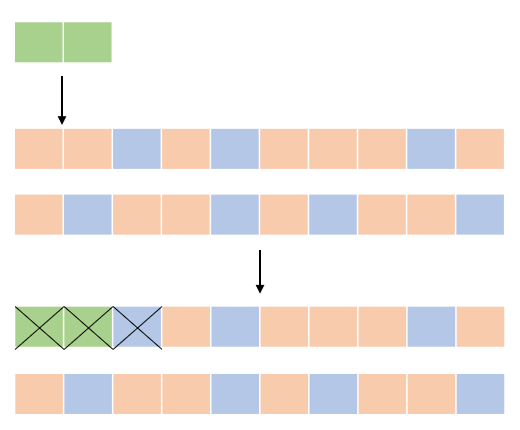
\includegraphics[width=5cm]{./Figures/seat_assign1.png}
%     \caption{Assign The Group in Row 1}
%     \end{minipage}
%     \begin{minipage}[t]{0.48\textwidth}
%     \centering
%     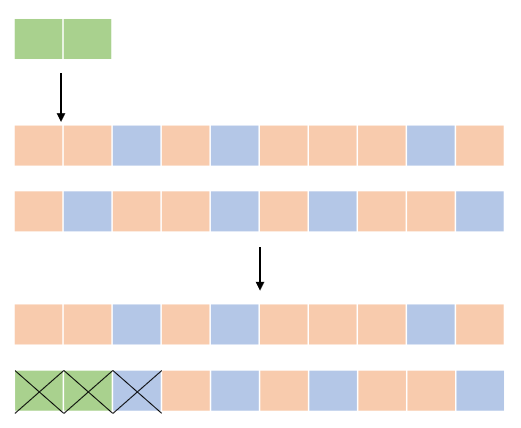
\includegraphics[width=5cm]{./Figures/seat_assign2.png}
%     \caption{Assign The Group in Row 2}
%     \end{minipage}
% \end{figure}


Our main contributions in this paper are summarized as follows. First, this study presents the first attempt to consider the arrangement of seat assignments with social distancing under dynamic arrivals. While many studies in the literature highlight the importance of social distancing in controlling the spread of the virus, they often focus too much on the model and do not provide much insight into the operational significance behind social distancing \cite{barry2021optimal, fischetti2021safe}. Recent studies have explored the effects of social distancing on health and economics, mainly in the context of aircraft \cite{salari2020social, ghorbani2020model, salari2022social}. Our study provides a new perspective to help the government adopt a mechanism for setting seat assignments to implement social distancing during pandemic.

Second, we establish a deterministic model to analyze the effects of social distancing when the demand is known. Due to the medium size of the problem, we can solve the IP model directly. We then develop the scenario-based stochastic programming by considering the stochastic demands of different group types. By using Benders decomposition methods, we can obtain the seat planning quickly. 

Third, to address the problem in the dynamic situation, we first obtain a feasible seat planning from scenario-based stochastic programming. We then make a decision for each incoming group based on our dynamic seat assignment policy, either accepting or rejecting the group. Our results demonstrate a significant improvement over the traditional control policies and provide the insights on the implementation of social distancing.

% Our results demonstrate the effectiveness of our approach in balancing social distancing requirements with revenue generation, providing valuable insights for policymakers and venue managers. Specifically, our proposed approach can help cinemas, concert venues, and other public spaces optimize seat assignments while ensuring the safety of patrons. It provides a practical tool for venues to implement social distancing measures in a flexible and efficient manner, adapting to changes in demand and maximizing revenue generation while maintaining social distancing measures.

% With this new .., we illustrate how to assign the seats by the govenment/stakeholder to balance health and economic issues. In addition, we also provide managerial guidance for the government on how to publish the related policy to make the tradeoff between economic maintenance and risk management.

The rest of this paper is structured as follows. The following section reviews relevant literature. We describe the motivating problem in Section 3. In Section 4, we establish the stochastic model,analyze its properties and obtain the seat planning. Section 5 demonstrates the dynamic seat assignment policy to assign the seats for incoming groups. Section 6 gives the numerical results and the insights of implementing social distancing. The conclusions are shown in Section 7.
\newpage


% !TEX root = sum1.tex
\section{Literature Review}\label{literature}

%The present study is closely connected to the following research areas: seat management with social distancing, multiple knapsack problem and network revenue management. The subsequent sections review the literature on each perspective and highlight significant differences between the present study and previous research.

%\subsection{Seating Management with Social Distancing}
Seating management is a practical problem that presents unique challenges in various applications, each with its own complexities, particularly when accommodating group-based seating requests. For instance, in passenger rail services, groups differ not only in size but also in their departure and arrival destinations, requiring them to be assigned consecutive seats \citep{clausen2010off, deplano2019offline}. In social gatherings such as weddings or dinner galas, individuals often prefer to sit together at the same table while maintaining distance from other groups they may dislike \citep{lewis2016creating}. In parliamentary seating assignments, members of the same party are typically grouped in clusters to facilitate intra-party communication as much as possible \citep{vangerven2022parliament}. In e-sports gaming centers, customers arrive to play games in groups and require seating arrangements that allow them to sit together \citep{kwag2022optimal}.

Incorporating social distancing into seating management has introduced an additional layer of complexity, sparking a new stream of research. Some works focus on the layout design and determine seating positions to maximize physical distance between individuals, such as students in classrooms \citep{bortolete2022support} or customers in restaurants and beach umbrella arrangements \citep{fischetti2023safe}. Other works assume the seating layout is fixed, and assign seats to individuals while adhering to social distancing guidelines. Examples include problems in air travel \citep{ghorbani2020model} and long-distance train travel \citep{haque2022optimization}. These studies underscore the growing relevance and importance of seating management in the context of social distancing.


Our work relates to seating management with social distancing for group-based requests, which has found its applications in various areas, including airplanes \citep{salari2022social}, trains \citep{haque2023social}, and theaters \citep{blom2022filling}. Due to the diversity of applications, there are different issues to handle. For example, in \cite{salari2022social}, the distance between different groups is taken into account, leading to the development of a seating assignment strategy that outperforms the simplistic airline policy of blocking all middle seats. In \citet{haque2023social}, when designing seat allocation for groups with social distancing, not only was the transmission risk inside the train considered, but also the transmission risk between different cities where the stops were located.


Our work is most closely related to \citet{blom2022filling}, as both address group-based seating problem in theaters. While in \citet{blom2022filling}, they primarily focus on scenarios with known groups - referred to as seat planning with deterministic requests in our work - we consider a broader range of demand patterns. Specifically, we also examine group-based seat planning with stochastic requests. We also consider dynamic seat assignment, assuming that groups arrive sequentially according to a stochastic process. 


%\subsection{Multiple Knapsack Problem}
When all requests are known, our problem is a special case of the multiple knapsack problem (MKP) \citep{pisinger1999exact}. It follows that some theoretical properties of MKP can be applied. However, in our problem, the knapsacks can have different capacities and there are many identical groups of the same size, thus, the aggregation form would be useful to obtain the seat plan. Furthermore, seat planning to utilize all seats is a crucial aspect of our analysis, which shows that our proposed approach will be different from those in the literature. 

% To address stochastic demand, we propose a scenario-based programming approach \cite{feng2013scenario, casey2005scenario, henrion2018problem} to determine the seat plan. Unlike existing literature, which typically considers the total supply for different demands or treats each type of supply as a protection level for corresponding demand types, we introduce a hierarchical consumption mechanism for the aggregated supply. Specifically, we adapt the constraints to reflect the hierarchical utilization of seats, where seats planned for larger groups can be repurposed for smaller groups. Additionally, the seat plan derived under demand uncertainty can serve as a reference for dynamic seat assignment, enhancing flexibility and effectiveness in real-time decision-making.

% {\bf not sure how to revise, remaining}

SADDP falls under the category of the dynamic multiple knapsack problem. When there is only one row, the problem reduces to the dynamic knapsack problem \citep{kleywegt1998dynamic}. However, there is limited research on the dynamic multiple knapsack problem, with only one mildly related study \citep{perry2009approximate}. This study models a multiperiod, single-resource capacity reservation problem by using multiple knapsacks to represent multiple time periods, which differs from our focus on the realistic multiple knapsack problem in seat assignment.

%\subsection{Network Revenue Management}
Our work is also related to the group-based \textit{network revenue management} (NRM) problem, which focuses on deciding whether to accept or reject a request \citep{gallego1997multiproduct}. The NRM problem can be fully characterized by a dynamic programming (DP) formulation. However, a significant challenge arises because the number of states grows exponentially with the problem size, rendering direct solutions computationally infeasible. To address this, various approaches have been proposed, such as deriving bid-price or booking-limit controls from static formulations or approximating the value function using simplified structures.

\citet{talluri1998analysis} was the first to propose bid-price control policies. Since then, a significant body of literature has focused on deriving refined bid prices and tighter bounds on value functions. In our work, we also consider a bid-price control policy, similar to the certainty equivalence control policy proposed by \citet{bertsimas2003revenue}, which directly uses the optimal value from a static model to approximate the initial value function. The seminal contribution to booking-limit control is from \citet{gallego1997multiproduct}, which studied a static model and introduced make-to-stock and make-to-order policies. However, these policies lack flexibility in handling stochastic demand and do not perform well for the group-based problem.


One of the key characteristics of our problem is that decisions must be made on an all-or-none basis for each group, which introduces additional complexity in handling group arrivals \citep{talluri2006theory}. Similar group-based characteristics are also observed in multi-day stays in hotel revenue management \citep{aydin2018decomposition, bitran1995application}, though the concept of a ``group'' in those contexts differs from our problem.

The introduction of group-based characteristics complicates seat management when using traditional bid-price and booking-limit control policies. Notably, in our model, the supply planned for larger groups can also be utilized by smaller groups. This flexibility stems from our approach, which focuses on group arrivals rather than individual units, distinguishing it from traditional partitioned and nested approaches \citep{curry1990optimal, van2008simulation}.

Another key characteristic of our study is the importance of seat assignment, which distinguishes it from traditional revenue management. The assign-to-seat feature introduced by \citet{zhu2023assign} further emphasizes the significance of seat assignment. This approach tackles the challenge of selling high-speed train tickets, where each request must be assigned to a specific seat for the entire journey. However, this paper focuses on individual passengers rather than groups, which sets it apart from our research.

\newpage


\section{Online MMKP}\label{sec_dynamic_seat}
Consider a set $\mathcal{N} = \{1, 2, \ldots, N\}$ of knapsacks, where each knapsack $j$ has a capacity $c_j \in \mathbb{Z}^{+}$. There is also a set $\mathcal{M} = \{1, 2, \ldots, M\}$ of distinct item types. Each item of type $i$ has a size $w_i \in \mathbb{Z}^{+}$ and yields a profit $r_i \in \mathbb{Z}^{+}$ when placed entirely into a knapsack. The item types are ordered such that their profit-to-weight ratios, $r_i / w_i$, are monotonically increasing in $i$.

Requests for these items arrive sequentially. Upon the arrival of a request (which specifies its type), the seller must immediately decide whether to accept or reject it. If accepted, the seller must also assign it to a specific knapsack with sufficient remaining capacity. Each item must be placed whole into a single knapsack; partial assignments or reassignments are not permitted.


To model this problem, we adopt a dynamic programming framework based on discrete time periods $t = 1, 2, \ldots, T$. In each period, at most one request arrives. Let $\lambda_i^t$ denote the probability that a request for an item of type $i \in \mathcal{M}$ arrives at time $t$. These probabilities satisfy $\sum_{i=1}^M \lambda_i^t \leq 1$ for all $t$, and we define $\lambda_0^t = 1 - \sum_{i=1}^M \lambda_i^t$ as the probability of no arrival in period $t$. Arrival events are assumed to be independent across time periods.


The system state is the vector of remaining capacities $\mathbf{C} = (c_1, \ldots, c_N)$. When an item of type $i$ arrives, the seller chooses a decision variable $u_{i,j}^t \in \{0,1\}$ for each knapsack $j$. The feasible set $U^t(\mathbf{C})$ is defined by:

$$
U^t(\mathbf{C})=\left\{u_{i, j}^t \in\{0,1\} \left\lvert\, \begin{array}{ll}
\text { (a) } & \sum_{j=1}^N u_{i, j}^t \leq 1 \quad \forall i \in \mathcal{M} \\
\text { (b) } & w_i u_{i, j}^t \leq c_j \quad \forall i \in \mathcal{M}, \forall j \in \mathcal{N}
\end{array}\right.\right\} .
$$

Constraint (a) ensures the item is assigned to at most one knapsack. Constraint (b) ensures that if the item is assigned to knapsack $j$ ($u_{i,j}^t=1$), its weight $w_i$ does not exceed $c_j$. The original vector form of this constraint, $w_{i}u_{i,j}^{t}\mathbf{e}_j \leq \mathbf{C}$ (where $\mathbf{e}_j$ is the $j$-th standard basis vector), is mathematically equivalent to (b).



Let $v^{t}(\mathbf{C})$ denote the value function, representing the maximum expected revenue obtainable from period $t$ onward, given the current remaining capacity vector $\mathbf{C}$. The Bellman equation is given by:

\begin{equation}\label{DP}
v^{t}(\mathbf{C}) = \max_{u_{i,j}^{t} \in U^{t}(\mathbf{C})}\left\{\sum_{i=1}^{M} \lambda_i^{t} \bigl( \sum_{j=1}^{N} r_i u_{i,j}^{t} + v^{t+1}(\mathbf{C} - w_i u_{i,j}^{t}\mathbf{e}_j)\bigr) + \lambda_0^{t} v^{t+1}(\mathbf{C})\right\}
\end{equation}

The boundary condition is $v^{T+1}(\mathbf{C}) = 0$ for all $\mathbf{C} \geq \mathbf{0}$, indicating that no more revenue can be earned after the final period $T$.

Let $\mathbf{C}_0 = (C_1, C_2, \ldots, C_N)$ be the initial capacity vector. The objective is to compute $v^{1}(\mathbf{C}_0)$, the maximum total expected revenue over the entire horizon from $t=1$ to $t=T$, and to find the policy of item assignments that achieves this value.


Solving the dynamic programming problem presented in Equation \eqref{DP} is computationally intractable for realistic problem sizes due to the curse of dimensionality inherent in the large state space.

To overcome this challenge, we propose a heuristic assignment policy. We first outline a traditional bid-price control policy. We then enhance this approach by introducing a novel bid-price control policy that leverages patterns.



% For any policy $\pi$, let $V^{\pi}$ denote the expected revenue collected under $\pi$. Among all policies, a special one is the dynamic programming (DP) policy as it achieves the maximal expected revenue. Apart from DP, another special policy is the hindsight optimum (HO), where the decision maker has full information on the demand realization for the entire time horizon and optimizes over the allocation schemes. Here, it is impossible for the HO to be attained because we can never know the full demand realization ahead. For ease of analysis, the hindsight optimum for the sample path is computed by solving a relaxed static problem and $V^{\text{HO}}$ is the expected value over all sample paths. Then for any online policy $\pi$, we have $$V^{\text{HO}} \geq V^{\text{DP}} \geq V^{\pi}.$$ It is well known that DP, despite its optimality, is computationally complex owing to the ``curse of dimensionality.'' Thus we use HO as our benchmark to evaluate the performance of any policy $\pi$.


\subsection{BPC Policy}
Bid-price control is a classical and widely studied methodology in network revenue management. The core idea is to set thresholds, known as bid prices, that represent the opportunity cost of consuming one unit of capacity. An item is accepted only if its revenue exceeds the estimated opportunity cost of the capacity it requires.

Typically, these bid prices are derived from the shadow prices of the capacity constraints in a deterministic approximation of the underlying stochastic problem. In this section, we detail the implementation of a bid-price control policy for our model.

We begin by formulating a deterministic linear programming (LP) approximation, specifically the LP relaxation of a multi-type multiple knapsack problem. This model uses expected demand over the horizon. Let $x_{ij}$ denote the number of type $i$ items assigned to knapsack $j$, and let $d_i = \sum_{t=1}^{T} \lambda^{t}_{i}$ represent the expected number of requests for type $i$. The formulation is as follows:


\begin{align}
\quad \max \quad & \sum_{i=1}^{M}  \sum_{j= 1}^{N} r_{i} x_{ij} \label{e0} \\
\text {s.t.} \quad & \sum_{j= 1}^{N} x_{ij} \leq d_{i}, \quad i \in \mathcal{M}, \label{deter_upper}\\ 
& \sum_{i=1}^{M} w_{i} x_{ij} \leq c_j, j \in \mathcal{N}, \label{capa_con} \\
& x_{ij} \geq 0, \quad i \in \mathcal{M}, j \in \mathcal{N}. \notag
\end{align}

The objective \eqref{e0} is to maximize total expected revenue. Constraint \eqref{deter_upper} ensures the total number of accepted type $i$ items does not exceed its expected demand. Constraint \eqref{capa_con} ensures the total weight in each knapsack $j$ does not exceed its initial capacity $C_j$.

The monotonic increase of the profit-to-weight ratio $r_i/w_i$ with type index $i$ implies that items with a higher index are more profitable per unit of capacity. Consequently, the optimal solution to the LP relaxation exhibits a greedy structure, preferentially utilizing higher-indexed item types. This structural property is formalized in Proposition \ref{sol_relax_deter}.

\begin{lem}\label{sol_relax_deter}
For the LP relaxation of the \textup{MMKP} problem, there exists an index $\tilde{i}$ such that the optimal solutions satisfy the following conditions: $x_{ij}^{*} = 0$ for all $j$, $i = 1,\ldots, \tilde{i}-1$; $\sum_{j=1}^{N} x_{ij}^{*} = d_{i}$ for $i = \tilde{i}+1,\ldots, M$; $\sum_{j=1}^{N} x_{ij}^{*} = \frac{L - \sum_{i = \tilde{i}+1}^{M} {d_i w_i}}{w_{\tilde{i}}}$ for $i = \tilde{i}$.
\end{lem}

The dual of LP relaxation of the MMKP problem is:

\begin{equation}\label{bid-price_dual}
    \begin{aligned}
    \min \quad & \sum_{i=1}^{M} d_i z_i + \sum_{j= 1}^{N} c_j \beta_{j} \\
    \text {s.t.} \quad & z_{i} + \beta_j w_i \geq r_i, \quad i \in \mathcal{M}, j \in \mathcal{N} \\
    & z_{i} \geq 0, i \in \mathcal{M}, \beta_{j} \geq 0, j \in \mathcal{N}.
    \end{aligned}
  \end{equation}

In \eqref{bid-price_dual}, $\beta_{j}$ can be interpreted as the bid-price for one size in knapsack $j$. A request is only accepted if the revenue it generates is no less than the sum of the bid prices of the sizes it uses. Thus, if $r_i -\beta_{j} w_i \geq 0$, meanwhile, the capacity allows, we will accept the item type $i$. And choose knapsack $j^{*} = \arg \max_{j} \{r_i -\beta_{j} w_i\}$ to allocate that item.

\begin{prop}\label{bid-price}
The optimal solution to problem \eqref{bid-price_dual} is given by $z_1 = \ldots = z_{\tilde{i}} =0$, $z_{i} = \frac{r_{i} w_{\tilde{i}} - r_{\tilde{i}} w_{i}}{w_{\tilde{i}}}$ for $i = \tilde{i}+1, \ldots, M$ and $\beta_j = \frac{r_{\tilde{i}}}{w_{\tilde{i}}}$ for all $j$.
\end{prop}

According to Proposition \ref{bid-price}, the decision inequality becomes $r_i -\beta_{j} w_i = r_{i} - \frac{r_{\tilde{i}}}{w_{\tilde{i}}} w_{i} \geq 0$. This establishes the threshold policy: reject item type $i, i < \tilde{i}$ and accept item type $i, i \geq \tilde{i}$.

\begin{algorithm}[H]
    \caption{Bid-Price Control}\label{algo_bid}
    \For{$t = 1, \ldots, T$}{
      {Observe a request of item type $i$\;}
      {Solve problem \eqref{bid-price_dual} with $\bm{d}^{[t,T]}$ and $\mathbf{C}^{t}$\;
      Obtain $\tilde{i}$ such that the aggregate optimal solution is $x e_{\tilde{i}} + \sum_{i=\tilde{i}+1} ^{M} d_{i}^{t} e_{i}$\;}
      \eIf{$i \geq \tilde{i}$ and $\max_{j \in \mathcal{N}}{c_j^{t}} \geq w_i$}
      {Set $k = \arg \min_{j \in \mathcal{N}}\{c_j^{t}|c_j^{t} \geq w_i\} $ and break ties\;
      Assign the item to knapsack $k$, let $c_{k}^{t+1} \gets c_{k}^{t} - w_{i}$ \;}
      {Reject the request\;}}
\end{algorithm}

% Let $val_{\theta}(I; \{d_{i}\})$ denote the optimal objective value of \eqref{theta_deter}.

% \begin{align}
%     \quad \max \quad & \sum_{i=1}^{M}  \sum_{j= 1}^{N} (n_i - \delta) x_{ij} \label{theta_deter} \\
%     \text {s.t.} \quad & \sum_{j= 1}^{N} x_{ij} \leq d_{i}, \quad i \in \mathcal{M}, \notag \\ 
%     & \sum_{i=1}^{M} n_{i} x_{ij} \leq \theta L_j, j \in \mathcal{N}, \notag 
% \end{align}

% Let $V_{\theta}^{OPT}(I)$ denote the expected value under optimal policy (relaxed) during $\theta T$ periods for instance $I$ (probability distribution).

% $V_{\theta}^{OPT}(I) = E_{\{d_{i}\}} [val_{\theta}(I; \{d_{i}\})] \leq val_{\theta} (I; \{E[d_{i}]\}) = val_{\theta}(I; \{\theta T p_{i}\})$

Let $z(\text{BPC})$, $z(\text{DLP})$ denote the optimal value of \eqref{bid-price_dual} and the LP relaxation of the \textup{MMKP} problem with expected demand, respectively. Then we have $z(\text{BPC}) = z(\text{DLP})$.

However, the BPC policy has two drawbacks. First, the capacity feasibility need to be checked when to accept a request. Second, when capacities permit, the policy treats all knapsacks as equally preferable, making no distinction among them.

\begin{example}
Consider an instance with $M =3$, $N =4$, $w_{1} = 3, w_{2} = 4, w_{3} = 5$, $r_{1} = 4, r_{2} = 6, r_{3} = 8$, $\bm{C} = [7, 8, 8, 4]$ and $T = 8$. The stationary arrival probability is $\lambda_{1} = \lambda_{3} = \frac{1}{4}$, $\lambda_{2} = \frac{1}{2}$, giving an expected demand vector $\bm{d} = (2, 4, 2)$.

Under traditional bid-price control, the bid-price for each knapsack $j$ is $\beta_{j}^{*} = \frac{4}{3}$, yielding a total expected reward $z(\text{BPC}) = \frac{124}{3}$. This solution exhibits two major drawbacks: 

It fails to differentiate between knapsacks, assigning them a uniform bid-price. It permits potentially infeasible assignments. For instance, even though $r_{3} - \beta_{4}^{*} * w_{3} > 0$, assigning a type 3 item (with weight 5) to knapsack 4 (with capacity 4) is infeasible.
\end{example}

\subsection{BPC Policy Based on Patterns (BPP)}
To better account for the differences between knapsacks when placing items, we propose an enhanced dynamic programming (DP) formulation. The key idea is to represent the state of each knapsack using feasible assignment patterns, which encode the combinations of items it can hold, rather than merely tracking its residual capacity. This approach more fully captures the knapsack's combinatorial structure.

Formally, a pattern for a knapsack is a vector $\bm{h} = [h_{1}, \ldots, h_{M}]$ where each $h_i$ denotes the number of type-$i$ items assigned. A pattern $\bm{h}$ is feasible for a knapsack with capacity $c_{j}$ if it satisfies $\sum_{i=1}^{M} w_{i} h_{i} \leq c_{j}$. We denote the set of all feasible patterns for knapsack $j$ by $S(c_{j})$. 

Let $v^t(\bm{C})$ denote the maximal expected value-to-go at time $t$, given the remaining capacity $\bm{C}$. The enhanced dynamic programming formulation is as follows:

\begin{equation}
v^t(\bm{C}) \geq \mathbb{E}_{i \sim \lambda^t}\left[\left\{
\begin{array}{ll}
\max \left\{\max\limits_{j:\bm{h} \in S(c_j), h_i \geq 1}\left\{v^{t+1}\left(\bm{C}-e_j^T \cdot w_i\right)+r_i\right\}, v^{t+1}(\bm{C})\right\},&\exists j, \text{satisfying} \bm{h} \in S(c_j), h_i \geq 1, \\
v^{t+1}(\bm{C}) & \text{otherwise}.
\end{array}\right]\right.
\end{equation}


The DP formulation involves two layers of maximization when there exists at least one knapsack $j$ satisfying $\bm{h} \in S(c_j), h_{i} \geq 1$. The inner maximization evaluates the optimal placement of item type $i$ across all feasible knapsacks $j$ where the pattern $\bm{h}$ is feasible for knapsack $j$ (i.e., $\bm{h} \in S(c_{j})$) and the item type $i$ can be accommodated (i.e., $h_{i} \geq 1$). The outer maximization compares the value of accepting $i$ (via the inner maximization) and rejecting $i$ (retaining $v^{t+1}(\bm{C})$). If no such $j$ exists, the request $i$ is rejected.


For notational convenience, we define $q_i$ as follows:
\begin{equation*}
    q_i= \begin{cases}\max _{j: \bm{h} \in S\left(c_j\right), h_i \geq 1}\left\{v^{t+1}\left(C-e_j^T w_i\right)+r_i\right\} & \text { if } \exists j \text{ satisfying } \bm{h} \in S\left(c_j\right), h_i \geq 1 \\ 0 & \text { otherwise }\end{cases}
\end{equation*}

We can solve the following program to compute $v^1(\bm{C})$ for any given capacity $\bm{C}$:

\begin{equation}\label{dp_bid}
    \begin{aligned}
    \min \quad & v^{1}(\bm{C}) \\
    \mathrm{s.t.} \quad & v^{t}(\bm{C}) \geq \mathbb{E}_{i \sim \lambda^t}\Bigg[\max\Big\{ q_{i}, v^{t+1}(\bm{C})\Big\}\Bigg], \\
    & v^{T+1}(\bm{C}) \geq 0.
    \end{aligned}
\end{equation}


Solving \eqref{dp_bid} remains computationally intractable. We therefore adopt an Approximate Dynamic Programming (ADP) approach \citep{adelman2007dynamic} to approximate the value function $v^{t}(\bm{C})$. Our proposed approximation is:

\begin{equation}\label{appro_dp}
    \hat{v}^{t}(\bm{C}) = \theta^{t} + \sum_{j=1}^{N} \max_{\bm{h} \in S(c_{j})} \{\sum_{i=1}^{M} \beta_{ij}^{\dag} h_{i}\}.
\end{equation}


The term $\beta_{ij}^{\dag}$ can be regarded as the approximated value for each type $i$ in knapsack $j$. Unlike traditional linear approximations, our approach retains the linear term $\theta^{t}$ but introduces a nonlinear component for each knapsack $j$. Specifically, we maximize the linear combination $\sum_{i=1}^{M} \beta_{ij}^{\dag} h_{i}$ over the feasible set $S(c_{j})$.

% Our approximation extends classical linear ADP by incorporating resource-specific nonlinear terms through constrained maximization over feasible allocations. While similar separable corrections appear in resource allocation ADP, our explicit use of $\max_{\bm{h} \in S(c_j)}$ captures local constraints more directly.


% Our approximation adopts a separable nonlinear structure, but unlike classical approximations, the nonlinearity is implicitly defined by constrained maximization over feasible allocations. This captures problem-specific constraints.

Substituting \eqref{appro_dp} into \eqref{dp_bid}, we have:

\begin{align}
    \theta^{t} - \theta^{t+1} = \hat{v}^{t}(\bm{C}) - \hat{v}^{t+1}(\bm{C}) \geq \sum_{i} \lambda_{i}^{t} \max\left\{q_{i} - v^{t+1}(\bm{C}), 0\right\}
\end{align}

For the case where there exists a knapsack $j$ satisfying both conditions: $\bm{h}^{*} \in \arg\max_{\bm{h} \in S(c_j)} \sum_{i} \beta_{ij}^{\dag} h_{i}$ and $h_{i}^{*} \geq 1$, we establish the value difference: 

\begin{align*}
    & v^{t+1}(\bm{C} - e_{j}^{T} w_{i}) - v^{t+1}(\bm{C}) \\ 
  = & \max_{\bm{h} \in S(c_{j}- w_{i})} \{\sum_{i} \beta_{ij}^{\dag} h_{i}\} - \max_{\bm{h} \in S(c_{j})} \{\sum_{i} \beta_{ij}^{\dag} h_{i}\} \\
  = & -\beta_{ij}^{\dag} \leq 0
\end{align*}

The acceptance threshold is then defined as:
$$\alpha_{i} = \max\left\{\max_{j}\left\{r_i - \beta_{ij}^{\dag} \right\}, 0\right\},$$ 
with $\alpha_{i} = 0$ when no qualifying knapsack $j$ exists.

Let $\gamma_{j} = \max_{\bm{h} \in S(c_{j})} \{\sum_{i} \beta_{ij}^{\dag} h_{i}\}$. This yields:

\begin{align*}
    \theta^{1} & = \sum_{t=1}^{T} (\theta^{t} - \theta^{t+1}) \geq \sum_{t} \sum_{i} \alpha_{i} \lambda_{i}^{t} = \sum_{i} d_{i} \alpha_{i} \\
    \hat{v}^{1}(\bm{C}) & = \sum_{i} d_{i} \alpha_{i} + \sum_{j} \gamma_{j}
\end{align*}

Since $\hat{v}^{1}(\bm{C})$ constitutes a feasible solution to \eqref{dp_bid}, we have $\hat{v}^{1}(\bm{C}) \geq v^{1}(\bm{C}) =  V^{DP}$.

If all $j$ exist for $\bm{h}^{*} \in \arg\max_{\bm{h} \in S(c_j)} \sum_{i} \beta_{ij}^{\dag} h_{i}, h_{i}^{*} \geq 1$, the corresponding bid-price problem can be expressed as:

\begin{equation}\label{improve_bid}
    \begin{aligned}
    \min \quad & \sum_{i=1}^M \alpha_i d_i+ \sum_{j=1}^N \gamma_j \\
    \mathrm{s.t.} \quad & \alpha_i+ \beta_{ij}^{\dag} \geq r_i, \quad \forall i, j, \\
    & \sum_{i=1}^M \beta_{ij}^{\dag} h_i \leq \gamma_j, \quad \forall j, \bm{h} \in S(c_j), \\
    & \alpha_i \geq 0, \forall i, \quad \beta_{ij}^{\dag} \geq 0, \forall i, j \\
    & \gamma_j \geq 0, \quad \forall j.
    \end{aligned}
\end{equation}

$\alpha_{i}$ represents marginal revenue for type $i$. $\beta_{ij}^{\dag}$ represents the cost for type $i$ assigned in knapsack $j$. $\gamma_{j}$ represents the capacity cost associated with knapsack $j$.

If for a given item type $i$, no knapsack $j$ contains an optimal allocation $\bm{h}^{*} \in \arg\max_{\bm{h} \in S(c_j)} \sum_{i} \beta_{ij}^{\dag} h_{i}$ with $h_{i}^{*} \geq 1$, then the variable $\alpha_{i}$ must be zero. This indicates that the constraint associated with item type $i$ and knapsack $j$ is redundant. Although these constraints appear difficult to enforce in advance, the following lemma reveals that in practice we can avoid imposing additional restrictions. Simply solving problem \eqref{improve_bid} will inherently satisfy all required conditions.

% \begin{lem}
% For the optimal solution, $r_{i} \geq \beta_{ij}^{\dag}$.
% \end{lem}

\begin{lem}\label{BPP}
Define $\mathcal{J}_{i} = \{j \in \mathcal{N} \mid r_i - \beta_{ij}^{\dag *} \geq r_i - \beta_{ik}^{\dag *},\forall k \in \mathcal{N}, r_i - \beta_{ij}^{\dag *} >0 \}$.
If $\mathcal{J}_{i} = \varnothing$, the first set of constraints for $i$ is redundant.
If $\mathcal{J}_{i} \neq \varnothing$, then there exists a $j{'} \in \mathcal{J}_{i}$ such that:

$$\bm{h}^{*} \in \arg\max_{\bm{h} \in S(c_{j{'}})} \sum_{i} \beta_{ij{'}}^{\dag *} h_{i}, h_{i}^{*} \geq 1.$$
\end{lem}

This lemma guarantees that when such a $j{'}$ exists, the first set of constraints for $i$ becomes active; otherwise, it remains inactive. Consequently, we have $z(\text{BPP}) = \hat{v}^{1}(\bm{C})$.

The control policy is then defined as follows. For the arriving type-$i$ item, if $\alpha_{i} > 0$, accept the type $i$. Assign the type $i$ to a knapsack $j \in \mathcal{J}_{i}$ satisfying: $$\bm{h}^{*} \in \arg\max_{\bm{h} \in S(c_j)} \sum_{i} \beta_{ij}^{\dag *} h_{i}, h_{i}^{*} \geq 1.$$ If $\alpha_{i} = 0$ and there exists a knapsack $j$ such that: $\bm{h}^{*} \in \arg\max_{\bm{h} \in S(c_j)} \sum_{i} \beta_{ij}^{\dag *} h_{i}, h_{i}^{*} \geq 1$, accept the type $i$ and assign it to knapsack $j$; otherwise, reject the type $i$.

Let $z(\text{BPC})$ and $z(\text{BPP})$ denote the expected optimal value of \eqref{bid-price_dual} and \eqref{improve_bid}, respectively.

\begin{prop}\label{BPC_relation}
    We have $z(\text{BPC}) \geq z(\text{BPP})$.
\end{prop}
    
% For the optimal $\beta_{j}^{*}$ in \eqref{bid-price_dual}, there exist optimal $\beta_{ij}^{\dag *}$ in \eqref{improve_bid} satisfying $\beta_{ij}^{\dag *} \geq w_{i} \beta_{j}^{*}$ for all $i$. 

% $\beta_{ij}^{\dag} = w_{i} \beta_{j}$ is feasible for \eqref{improve_bid}, then the optimal bid-price 
    
Both bid-price approaches give upper bounds on the value function at any state, meanwhile it follows that BPP provides a tighter approximation to the value function more accurately than BPC does.

Under the approximation \eqref{appro_dp}, the BPP policy operates as follows:

% accept type $i$ if $r_i - \beta_{ij}^{\dag} > 0$ and at least one knapsack can assign type $i$, check  item type $i$ otherwise. 

% $\max_{j \in \mathcal{N}}{c_j^{t}} \geq w_i$

\begin{algorithm}[H]
    \caption{Bid-Price Control Based on Patterns}\label{algo_improve_bid}
    \For{$t =1, \ldots, T$}{
      {Observe a request of item type $i$\;}
      {Solve problem \eqref{improve_bid} with $\bm{d}^{[t, T]}$ and $\mathbf{L}^{t}$\;}
      \eIf{$\alpha_i > 0$}
      {Assign the type $i$ to a knapsack $j \in \mathcal{J}_{i}$ satisfying: $$\bm{h}^{*} \in \arg\max_{\bm{h} \in S(c_j)} \sum_{i} \beta_{ij}^{\dag *} h_{i}, h_{i}^{*} \geq 1.$$
      Let $c_{j}^{t+1} \gets c_{j}^{t} - w_{i}$\;}
      {\eIf{There exists $j$ such that $\bm{h}^{*} \in \arg\max_{\bm{h} \in S(c_j)} \sum_{i} \beta_{ij}^{\dag} h_{i}, h_{i}^{*} \geq 1$}{Assign the item in knapsack $j$, let $c_{j}^{t+1} \gets c_{j}^{t} - w_{i}$\;}
      {Reject the request\;}}}
\end{algorithm}

% Furthermore, the BPP policy exhibits a threshold structure similar to the BPC policy. There exists a threshold type $\tilde{i}$ (or $\tilde{i}-1$, depending on the remaining capacity and expected future demand) such that all item types $i \leq \tilde{i}$ (or $i \leq \tilde{i}-1$) are rejected and larger types $i > \tilde{i}$ (or $i > \tilde{i}-1$) are accepted.

% Specifically, we have 
% \begin{lem}\label{BPP_decision}    
%     For the threshold index $\tilde{i}$ in Proposition \ref{sol_relax_deter},
%     \begin{itemize}
%         \item If $\sum_{i=\tilde{i}}^{M} d_{i} w_{i} > \sum_{j=1}^{N} c_{j}$, then $r_i - \beta_{ij}^{\dag} \leq 0$, for $i \leq \tilde{i}$,
%         \item If $\sum_{i=\tilde{i}}^{M} d_{i} w_{i} = \sum_{j=1}^{N} c_{j}$, then $r_i - \beta_{ij}^{\dag} \leq 0$, for $i \leq \tilde{i}-1$.
%     \end{itemize}
% \end{lem}

% Lemma \ref{BPP_decision} indicates how the relation between the remaining capacity and the expected demand affects the decision.

% when $\sum_{i=\tilde{i}}^{M} d_{i} w_{i} > \sum_{j=1}^{N} c_{j}$, item type $i, i \leq \tilde{i}$ is rejected and item type $i, i > \tilde{i}$ is accepted; when $\sum_{i=\tilde{i}}^{M} d_{i} w_{i} = \sum_{j=1}^{N} c_{j}$, item type $i, i \leq \tilde{i}-1$ is rejected and item type $i, i \geq \tilde{i}$ is accepted.

% Proof:
% $\sum_{j} x_{ij}^{*} < d_{i}$, then $\alpha_{i}^{*} = 0$. $i - \beta_{ij}^{\dag} \leq 0$.

% Lemma \ref{BPC_relation} shows that the I-BPC policy does not uniformly reject all small groups. Instead, it selectively accepts them based on pattern-based allocation, enabling more flexible decision-making. Unlike the traditional BPC, the I-BPC policy accounts for row-specific characteristics in allocation decisions. Therefore, the I-BPC policy better captures the structure of the capacity than the BPC policy does.


Unlike the traditional BPC, the BPP does not require explicit feasibility checks on capacity. However, it still needs to verify whether the optimal pattern contains the given request. This introduces a new challenge, as bid-price policies are inherently derived from a dual formulation, which may inherently omit key information preserved in the primal problem.

\begin{example}
Continue with the above example:

For the BPP, the optimal bid price is $\bm{\beta}_{1}^{*} = [4, 4, 4, 6]$, $\bm{\beta}_{2}^{*} = [6, 6, 6, 6]$, $\bm{\beta}_{3}^{*} = [10, 8, 8, 8]$. We can verify that  $z(BPP) = 40 < z(BPC) = \frac{124}{3}$. The reduced reward for each item type 3 is: $r_{3} - \bm{\beta}_{3}^{*} = [-2, 0, 0, 0]$, which indicates type 3 is excluded from knapsack 1. Also, the optimal patterns for knapsack 4, $[0, 1, 0]$ and $[1, 0, 0]$. Thus, type 3 can only be assigned to knapsack 2 or 3.

% The corresponding primal variables are $\bm{\alpha} = [0, 0, 0]$ and $\bm{\gamma} = [10, 12, 12, 6]$.

% A drawback is that one must check if an item type can be assigned to a knapsack $j_0$ by verifying the condition $\bm{h}^{*} \in \arg\max_{\bm{h} \in S(c_{j_0})} \sum_{i} \beta_{ij_0}^{\dag *} h_{i}$ with $h_{i}^{*} \geq 1$.


\end{example}

While this verification is cumbersome under pure bid-price frameworks, the primal problem offers a more direct way to guarantee the existence of such a request-pattern match. To address this gap, we propose the dynamic primal formulation.

\section{Dynamic Primal Based on Patterns}

Let $y_{j \bm{h}}$ denote the proportion of pattern $\bm{h}$ used in knapsack $j$. The primal problem can be formulated as:

\begin{equation}\label{improve_primal}
    \begin{aligned}
    \max \quad & \sum_{i=1}^M \sum_{j=1}^N r_i x_{i j} \\
    \text {s.t.} \quad & \sum_{j=1}^N x_{i j} \leq d_i, \quad i \in \mathcal{M}, \\
    & x_{i j} \leq \sum_{\bm{h} \in S(c_{j})} h_i y_{j \bm{h}}, \quad i \in \mathcal{M}, j \in \mathcal{N}, \\
    & \sum_{\bm{h} \in S(c_{j})} y_{j \bm{h}} \leq 1, \quad j \in \mathcal{N}.
    \end{aligned}
\end{equation}

The first set of constraints demonstrate that for each item type $i$, the sum of assigned items and unassigned items equals the total demand. The second set of constraints shows that the number of items of type $i$ assigned in knapsack $j$ is not larger than the sum of $h_{i}$ (the count of type $i$ items in pattern $\bm{h}$) weighted by the pattern proportions $y_{i \bm{h}}$. The total proportion of patterns uesd in knapsack $j$ cannot exceed 1.

\begin{prop}\label{primal}
If the optimal solution $x_{ij}^{*}$ to \eqref{improve_primal} satisfies $x_{ij}^{*} > 0$ for a pair $(i,j)$, then for that knapsack $j$, we have $$\bm{h}^{*} \in \arg\max_{\bm{h} \in S(c_j)} \sum_{i} \beta_{ij}^{\dag} h_{i}, h_{i}^{*} \geq 1.$$
\end{prop}

In contrast to Lemma \ref{BPP}, this lemma ensures the existance of a knapsack $j$ to accommodate item type $i$ when $x_{ij}^{*} > 0$. This eliminates the need for explicit existance verification.

% Then, the following hierarchy holds: $V(\text{DLP}) = V(\text{BPC}) \geq V(\text{I-BPC}) \geq V^{\text{DP}}$.

% Any feasible solution to \eqref{improve_primal} yields a feasible solution to linear relaxation of SPDR having the same objective value, then we have  $V(\text{BPC}) \geq V^{\text{HO}} \geq V^{\text{DP}}$.



\subsection{Solve the Dynamic Primal}
% A pattern $\bm{h}$ is said to be inefficient if a mixture of other patterns can be used to generate more revenue for the same (or lower) consumption rate.

The pattern $\bm{h}$ is efficient for knapsack $j$ if and only if, for some $(\alpha_{1}, \ldots, \alpha_{M}, \gamma_{j})$ (except that $\alpha_{i} = r_i, \forall i$), $\bm{h}$ is the optimal solution to $$\max_{\bm{h}} \sum_{i=1}^{M} (r_i - \alpha_{i}) h_{i} - \gamma_{j}$$

To generate all efficient patterns, we need to solve the subproblem for each knapsack $j$:

\begin{align}\label{subproblem}
    \max \quad & \sum_{i=1}^{M} (r_i - \alpha_{i}) h_{i} - \gamma_{j} \\
    \text {s.t.} \quad & \sum_{i= 1}^{M} w_{i} h_{i} \leq c_j, \notag \\
    & h_{i} \in \mathbb{N}, \quad i \in \mathcal{M}. \notag
\end{align} 

If the optimal value of \eqref{subproblem} is larger than $0$, the primal $\eqref{improve_primal}$ reaches the optimal. Otherwise, a new pattern can be generated.

One important fact is that only efficient sets are used in the solution to \eqref{improve_primal}. Therefore, if $y_{j \bm{h}}^{*} > 0$ is the optimal solution to \eqref{improve_primal}, then $\bm{h}$ is an efficient pattern.


A pattern $\bm{h}$ is dominant if there is no distinct pattern $\bm{h}{'}$ where every component of $\bm{h}{'}$ is greater than or equal to the corresponding component of $\bm{h}$. The efficient pattern is a dominating pattern. (If $\alpha_{i} = r_i$, \eqref{improve_primal} reaches the optimal and no pattern will be generated.)

The relation between the capacity and the demand shows the different structure of the optimal solution.

\begin{lem}
When $\sum_{i=1}^{M} d_{i} w_{i} < \sum_{j=1}^{N} c_{j}$, we have $\gamma_{j}^{*} =0, \forall j$, $\beta_{ij}^{\dag *} =0, \forall i,j$ and $\alpha^{*}_{i} = r_i, \forall i$. There exists at least one knapsack $j$ such that $\sum_{\bm{h} \in S(c_{j})} y_{j \bm{h}}^{*} < 1$.

When $\sum_{i=1}^{M} d_{i} w_{i} \geq \sum_{j=1}^{N} c_{j}$, we have $\sum_{\bm{h} \in S(c_{j})} y_{j \bm{h}}^{*} = 1, \forall j$.
\end{lem}


\begin{algorithm}[H]
    \caption{Dynamic Primal}\label{algo_improve_primal}
    \For{$t = 1, \ldots, T$}{
      {Observe a request of type $i$\;}
      \If{$c_{j}^{t} = w_i, \exists j$}
      {Assign the item to knapsack $j$\; 
      \Continue}
      {Solve problem \eqref{improve_primal} with $\bm{d}^{[t, T]}$ \;
      Obtain an optimal solution $x_{ij}$ \;}
      \eIf{$\max_{j}\{x_{ij}\} > 0$}
      {Set $k = \arg \max_{j}\{x_{ij}\}$ and break ties\;
      Assign the item to knapsack $k$, let $c_{k}^{t+1} \gets c_{k}^{t} - w_{i}$\;}
      {Reject the request\;}}
\end{algorithm}

Meanwhile, it guarantees feasible placement. Once a request is accepted, the policy ensures it can be assigned to a suitable knapsack without additional feasibility checks.

\begin{example}
For the dynamic primal, the optiaml solution is given by $\bm{x}_{1}^{*} = [1, 1, 0, 0]$, $\bm{x}_{2}^{*} = [1, 0, 2, 1]$, $\bm{x}_{3}^{*} = [0, 1, 0, 0]$. This indicates that type 1 can be assigned to knapsacks 1 or 2, type 2 cannot be assigned to knapsack 2, type 3 can only be assigned to knapsack 2. 

In the optimal solution, the efficient patterns for each knapsack are $[1, 1, 0]$, $[1, 0, 1]$, $[0, 2, 0]$, $[0, 1, 0]$. For instance, $[1, 1, 0]$ shows that knapsack 1 can hold one item of type 1 and one of type 2.

Using the decision variable $x_{ij}$ to represent these assignments is a straightforward and easily implementable approach.
\end{example}


% \begin{example}
% Consider $M =3$, $N =4$, $w_{1} = 3, w_{2} = 4, w_{3} = 5$, $r_{1} = 4, r_{2} = 6, r_{3} = 8$, $\bm{C} = [7, 8, 8, 4]$, $T = 8$, stationary arrival probability, $\lambda_{1} = \lambda_{3} = \frac{1}{4}$, $\lambda_{2} = \frac{1}{2}$. Then the expected demand for each type is $\bm{d} = (2, 4, 2)$.

% For the traditional bid-price control, for each $j$, $\beta_{j}^{*} = \frac{4}{3}$. $z(BPC) = \frac{124}{3}$. Two drawbacks: there is no difference among knapsacks. Even $r_{3} - \beta_{4}^{*} * w_{3} > 0$, it is infeasible for type 3 assigned in knapsack 4.

% For the BPP, $\bm{\beta}_{1}^{*} = [4, 4, 4, 6]$, $\bm{\beta}_{2}^{*} = [6, 6, 6, 6]$, $\bm{\beta}_{3}^{*} = [10, 8, 8, 8]$. $z(BPP) = 40$. $\alpha = [0, 0, 0]$, $\gamma = [10, 12, 12, 6]$.

% $r_{1} - \bm{\beta}_{1}^{*} = [0, 0, 0, -2]$, $r_{2} - \bm{\beta}_{2}^{*} = [0, 0, 0, 0]$, $r_{3} - \bm{\beta}_{3}^{*} = [-2, 0, 0, 0]$.

% Drawback: need to check whether $j$ exists for $\bm{h}^{*} \in \arg\max_{\bm{h} \in S(c_{j_0})} \sum_{i} \beta_{ij_0}^{\dag *} h_{i}, h_{i}^{*} \geq 1$.

% For example, $r_{3} - \bm{\beta}_{3}^{*} = [-2, 0, 0, 0]$ indicates type 3 cannot be assigned in knapsack 1. While the generated patterns for knapsack 4 are $[0, 1, 0], [1, 0, 0]$, which do not contain $h_{3}$, type 3 can only be assigned to knapsack 2 or 3.

% % $[1, 1, 0], [2, 0, 0], [0, 0, 1]$, $[0, 2, 0], [1, 0, 1]$, $[0, 2, 0], [1, 0, 1]$, $[0, 1, 0], [1, 0, 0]$

% For the primal, $\bm{x}_{1}^{*} = [1, 1, 0, 0]$, $\bm{x}_{2}^{*} = [1, 0, 2, 1]$, $\bm{x}_{3}^{*} = [0, 1, 0, 0]$. It indicates that type 1 can be assigned in knapsacks 1 or 2, type 2 cannot be assigned in knapsack 2, type 3 can only be assigned in knapsack 2. 

% It may contain multiple efficient patterns for one knapsack. In this example, there is exactly one efficient pattern for each knapsack: $[1, 1, 0]$, $[1, 0, 1]$, $[0, 2, 0]$, $[0, 1, 0]$. It shows that knapsack 1 can assign type 1 and 2, so on and so forth.

% Using $x_{ij}$ to make the decision is straightforward and easy to implement.
% \end{example}


% \subsection{Type Analyses}

% When there is only one type, the optimal policy is straightforward, i.e., accept the request until the capacity is insufficient. 

% When there are two types, 

% When will the threshold policy be the optimal?

% Applications.

% !TEX root = sum1.tex
\section{Asymptotic Loss}

% \begin{lem}
%     Loss: $\lim_{\theta \to \infty} V_{\theta}^{\text{DP}} - z_{\theta}({\text{BPC}}) = 0$. 
% \end{lem}

$\theta$ is the scale parameter.

\begin{prop}
    Loss: $V_{\theta}^{\text{HO}} - V_{\theta}^{\text{BL}} = O(\sqrt{\theta})$. 
\end{prop}

\begin{prop}
    Loss: $V_{\theta}^{\text{HO}} - V_{\theta}^{\text{P}} = O(1)$. 
\end{prop}

% Let $T_{i} = sup \{t \leq T: \lambda_{i}^{t} > 0\}$. 

% \newpage

\subsection{Loss for Static BLC Policy}
Booking limit control policy:

\begin{align}
    \quad \max \quad & \sum_{i=1}^{M}  \sum_{j= 1}^{N} r_{i} x_{ij} \label{theta_deter} \\
    \text {s.t.} \quad & \sum_{j= 1}^{N} x_{ij} \leq d_{i}, \quad i \in \mathcal{M}, \notag \\ 
    & \sum_{i=1}^{M} w_{i} x_{ij} \leq L_j, j \in \mathcal{N}, \notag 
\end{align}


Let $d_{i} =\sum_{t} \bm{1}_{i_{t} = i}$ be the realized number of type $i$ over the horizon $T$. 
Consider the deterministic linear programming \eqref{theta_deter}, where the right-hand side demands are set to $\sum_{t} \lambda_{i}^{t}$. Let $x_{ij}^{*}$ be an integral optimal solution to this LP, and define $d_{i}^{*} = \sum_{j} x_{ij}^{*}$ as the total number of type $i$ assigned in this optimal solution. Finally, let $val(I; \{d_{i}\})$ denote the optimal objective value of \eqref{theta_deter} for a given instance $I$ and demand vector $\{d_{i}\}$.

$V^{BL}(I) = E_{\{d_{i}\}}[\sum_{i} r_{i} \min\{d_{i}^{*}, d_{i}\}]$, $V^{OPT}(I) = E_{\{d_{i}\}} [val(I; \{d_{i}\})] \leq val(I; \{E[d_{i}]\})$.

$val(I; \{d_{i}\})$ is concave in $d_{i}$.

\begin{align*}
   & V^{OPT}(I) - V^{BL}(I) \\
\leq & val(I; \{E[d_{i}]\}) - V^{BL}(I) \\
= & val(I; \{E[d_{i}]\}) - val(I; \{\lfloor E[d_{i}]\rfloor\}) + val(I; \{\lfloor E[d_{i}]\rfloor\}) - E_{\{d_{i}\}}[\sum_{i} r_{i} \min\{d_{i}^{*}, d_{i}\}] \\
\leq & \sum_{i} r_{i} + N \sum_{i} r_i + E_{\{d_{i}\}}[\sum_{i} r_{i} (d_{i}^{*} - \min\{d_{i}^{*}, d_{i}\})] \\
= & (1+N) \sum_{i} r_{i} + E_{\{d_{i}\}}[\sum_{i} \frac{1}{2} r_{i} (d_{i}^{*} - d_{i} + |d_{i}^{*} - d_{i}|)] \\
\overset{\text{(a)}}{\leq} & (1+N) \sum_{i} r_{i} + \frac{1}{2} \sum_{i} r_{i} (d_{i}^{*} - E[d_{i}] + |d_{i}^{*} - E[d_{i}]| + \sqrt{\Var[d_{i}]}) \\
\leq & (1+N) \sum_{i} r_{i} + \frac{1}{2} \sum_{i} r_{i} \sqrt{\Var[d_{i}]} \\
\leq & (1+N) \sum_{i} r_{i} + \frac{1}{2} \sum_{i} r_{i} \sqrt{T p_{i} (1- p_{i})} = O(\sqrt{T})
\end{align*}

The revenue loss between the static deterministic heuristic and the optimal is bounded by $C \sqrt{T}$.
Thus, $\lim_{T \to \infty} (V^{OPT}(I) - V^{BL}(I))/T \to 0$.

$val(I; \{E[d_{i}]\}) - val(I; \{\lfloor E[d_{i}]\rfloor\}) \leq val(I; \{\lceil E[d_{i}]\rceil\}) - val(I; \{\lfloor E[d_{i}]\rfloor\}) \leq \sum_{i} r_{i}$


$LP -IP \leq \sum_{i} \sum_{j} r_{i} (x_{ij}^{*} - \lfloor x_{ij}^{*} \rfloor) < N \sum_{i} r_i$ $\Rightarrow$ $val(I; \{\lfloor E[d_{i}]\rfloor\}) \leq IP + N \sum_{i} r_i$.

$IP = \sum_{i} \sum_{j} r_{i} x_{ij}^{*} = \sum_{i} r_{i} d_{i}^{*}$

$(a)$ results from the following inequalities: $|d_{i}^{*} -d_{i}| = |(d_{i}^{*}-E[d_{i}]) + (E[d_{i}] -d_{i})| \leq |d_{i}^{*}-E[d_{i}]| + |d_{i} - E[d_{i}]|$. Take the expectation, we have $E[|d_{i}^{*} -d_{i}|]\leq |d_{i}^{*}-E[d_{i}]| + E[|d_{i} - E[d_{i}]|]$. $E[|d_{i} - E[d_{i}]|] \leq \sqrt{\Var[d_{i}]}$(Since $E[|X|] \leq \sqrt{E[X^{2}]}$). $d_{i}^{*} \leq E[d_{i}]$.

% 0-1 multiple

% \begin{align}
%     \quad \max \quad & \sum_{i=1}^{M}  \sum_{j= 1}^{N} p_i x_{ij} \\
%     \text {s.t.} \quad & \sum_{i= 1}^{M} w_{i} x_{ij} \leq L_{j}, \quad j \in \mathcal{N} \\ 
%     & \sum_{j=1}^{N} x_{ij} \leq 1, i \in \mathcal{M}  \\
%     & x_{ij} \in \{0,1\}, \quad i \in \mathcal{M}, j \in \mathcal{N}. 
% \end{align}

% Here, $M = \sum_{i=1}^{m} d_{i}$ represents the number of groups. $p_{k} = (n_{i} - \delta), w_{k} = n_{i}$ if group $k$ belongs to type $i$.


% single-leg RM: bid-price and booking limit expected revenue loss of $O(\sqrt{k})$ even with re-solving.


\subsection{Loss for Dynamic Primal Policy}

$E[\text{loss}] = V^{\text{off}} - V_{\pi}^{on} \geq V^{\text{opt}} - V_{\pi}^{on}$

Let $V^{\text{OPT}}(I)$ denote the expected value under offline optimal policy (relaxed) during $T$ periods for instance $I$ (capacity, probability distribution).


Let $\gamma_{ij}$, $\gamma_{i}^{0}$ denote the number of type $i$ accepted in capacity $j$ and rejected by this policy, respectively.


% Re-solving (each stage) bid-price (DLP) is equivalent to the optimal policy.
\begin{align*}
    OPT(\bm{C}, d, \gamma): \quad \max \quad & \sum_{i = 1}^{M} \sum_{j = 1}^{N} r_{i} x_{ij} \\
    \text {s.t.} \quad & \sum_{j=1}^{N} x_{ij} + x_{i0} = d_{i}, \quad i \in \mathcal{M},  \\ 
    & x_{ij} \geq \gamma_{ij}, \quad i \in \mathcal{M}, j \in \mathcal{N} \\
    & x_{i0} \geq \gamma_{i}^{0}, \quad i \in \mathcal{M}, \\
    & \sum_{i=1}^{M} w_{i} x_{ij} \leq c_{j}, \quad j \in \mathcal{N}.
\end{align*}


% At time $t$, solve the primal problem \eqref{improve_primal} with demands $d_{i} = \sum_{\tau = t}^{T} * \lambda_{i}^{\tau}$. If the resulting solution has $x_{i} > 0$ for the current request's type $i$, then accept the request.


$d^{[1, T]}$ is the demand realization during $[1, T]$. $\gamma_{ij}^{[1, t)}$ represents the number of requests $i$ assigned in knapsack $j$ by the policy during $[1, t)$.

$OPT(\bm{C}, d^{[1, T]}, \gamma^{[1,t+1)})$ can be interpreted as the total reward obtained under a virtual policy where we first follow the heuristic policy during $[1, t+1)$ and then from time $t+1$ we follow the optimal solution assuming that we know the future demands.

For one sample path of the requests, the revenue loss can be decomposed into $T$ increments.

\begin{align*}
    & OPT(\bm{C}, d^{[1, T]}, 0) - OPT(\bm{C}, d^{[1, T]}, \gamma^{[1, T]}) \\
 = & \sum_{t=1}^{T} [OPT(\bm{C}, d^{[1,T]}, \gamma^{[1,t)}) - OPT(\bm{C}, d^{[1,T]}, \gamma^{[1,t+1)})]
\end{align*}

% Let $c_{j}^{t} = c_{j} -\sum_{i=1}^{M} w_{i} \gamma_{ij}^{[1,t)}$. 

Let $T_{i} = \sup\{t \leq T: \lambda_{i}^{t}> 0\}$. 

Then 
$$
\inf_{\substack{t, i: \\ t \in\left[\theta T_{i}\right]}} \frac{\lambda_{i}^{\left(t, \theta T_{i}\right]}(\theta)}{\theta T_{i}-t}
$$

is lower bounded by some positive constant 
$$
\lambda_{\min } \triangleq \inf_{i} \frac{\lambda_{i}^{T_{i}}}{T_{i}}
$$


The expected revenue loss can be upper bounded:

\begin{align*}
    & E[OPT(\bm{C}, d^{[1, T]}, 0) - OPT(\bm{C}, d^{[1, T]}, \gamma^{[1, T]})] \\
 \leq & l \sum_{t=1}^{T} P(OPT(\bm{C}, d^{[1, T]}, \gamma^{[1,t)}) - OPT(\bm{C}, d^{[1, T]}, \gamma^{[1,t+1)}) > 0) \\
 = & l \sum_{t=1}^{T} P(OPT(\bm{C}^{t}, d^{[t, T]}, 0) - OPT(\bm{C}^{t}, d^{[t, T]}, \gamma^{[t,t+1)}) > 0) \\
 \leq & l \sum_{t=1}^{T} P(x_{i^{t}j^{t}}^{*,t} <1)
\end{align*}

$OPT(\bm{C}, d^{[1, T]}, \gamma^{[1,t)}) - OPT(\bm{C}, d^{[1, T]}, \gamma^{[1,t+1)}) \leq l$.
$l$ is related to $r_{M}$.

\begin{lem}\label{additive}
$OPT(\bm{C}^{1}, \hat{d} + d^{[1, t_2)} , \gamma^{[1, t_2)}) = \sum_{i} r_{i} \sum_{j} \gamma_{ij}^{[1, t_1)} + OPT(\bm{C}^{t}, \hat{d}+d^{[t_1, t_2)}, \gamma^{[t_1, t_2)})$
\end{lem}

For any optimal solution $x^{*}$ of $OPT(\bm{C}^{t}, \hat{d}+d^{[t_1, t_2)}, \gamma^{[t_1, t_2)})$, $x^{*} + \gamma^{[1, t_1)}$ is a feasible solution of $OPT(\bm{C}^{1}, \hat{d}+d^{[1, t_2)}, \gamma^{[1, t_2)})$. For any optimal solution $x^{*}$ of $OPT(\bm{C}^{1}, \hat{d}+d^{[1, t_2)}, \gamma^{[1, t_2)})$, $x^{*}- \gamma^{[1, t_1)}$ is a feasible solution of $OPT(\bm{C}^{t}, \hat{d}+d^{[t_1, t_2)}, \gamma^{[t_1, t_2)})$ because $x^{*}- \gamma^{[1, t_1)} \geq \gamma^{[1, t_{2})}- \gamma^{[1, t_1)} = \gamma^{[t_1, t_2)}$.


The first inequality results from $E[A] \leq l E[\bm{1}_{A>0}] = l P(A>0)$.

The first equation follows from Lemma \ref{additive}. (Let $t_1 = t_2 = t$, $\hat{d} = d^{[t, T]}$; let $t_1 = t, t_2 = t+1$, $\hat{d} = d^{[t+1, T]}$).

The second equation is as follows. If $x_{i^{t}j^{t}}^{*,t} \geq 1$, then $x^{*,t}$ is still feasible for $OPT(\bm{C}^{t}, d^{[t, T]}, \gamma^{[t,t+1)})$. (Because the optimal policy)

$x_{i^{t}j^{t}}^{*,t}$ is the optimal solution for $\text{OPT}(\bm{C}^{t}, d^{[t, T]}, 0)$ at time $t$.

Now we consider $P(x_{i^{t}j^{t}}^{*,t} <1)$. In time period $t$, after realization of $i^{t}$, based on the maximum choice of $j^{t}$ in dynamic primal policy, we have

$$
\gamma_{i^t j^t}^{\mathrm{P}, t}=\max_{j} \gamma_{i^t j}^{\mathrm{P}, t} \geqslant \frac{\sum_{j} \gamma_{i^t j}^{\mathrm{P}, t}}{\sum_{j} 1} = \frac{\lambda_{i^t}^{[t, \theta T]}}{N}
$$


$$
\begin{aligned}
& \mathbb{P}\left(x_{i^{t}j^{t}}^{*,t} <1\right) \\
\leqslant & \mathbb{P}\left(x_{i^{t}j^{t}}^{*,t} < x_{i^{t}j^{t}}^{\mathrm{P}, t}+1-\frac{\lambda_{i^t}^{[t, \theta T]}}{N}\right) \\
= & \mathbb{P}\left(x_{i^{t}j^{t}}^{\mathrm{P}, t} - x_{i^{t}j^{t}}^{*,t} > \frac{\mathbb{E}\left[d_{i^t}^{[t, \theta T]}\right]-N}{N}\right) \\
\stackrel{(\mathrm{a})}{\leqslant} & \mathbb{P}\left(\max_{i^{\prime}}\left|\mathbb{E}\left[d_{i^{\prime}}^{[t, \theta T]}\right]-d_{i^{\prime}}^{[t, \theta T]}\right|> \frac{\mathbb{E}\left[d_{i^t}^{[t, \theta T]}\right]-N}{\delta N} \right) \\
= & \mathbb{P}\left(\bigcup_{i^{\prime}}\left\{\left|\mathbb{E}\left[d_{i^{\prime}}^{[t, \theta T]}\right] - d_{i^{\prime}}^{[t, \theta T]}\right|> \frac{\mathbb{E}\left[d_{i^t}^{[t, \theta T]}\right]-N}{\delta N} \right\}\right) \\
\leqslant & \sum_{i^{\prime}} \mathbb{P}\left(\left|\mathbb{E}\left[d_{i^{\prime}}^{[t, \theta T]}\right]-d_{i^{\prime}}^{[t, \theta T]}\right|> \frac{\mathbb{E}\left[d_{i^t}^{[t, \theta T]}\right]-N}{\delta N}\right) \\
\stackrel{(\mathrm{b})}{=} & \sum_{i^{\prime}} \sum_{i} \mathbb{P}\left(\left.\left|\mathbb{E}\left[d_{i^{\prime}}^{[t, \theta T]}\right]-d_{i^{\prime}}^{[t, \theta T]}\right| > \frac{\mathbb{E}\left[d_{i^t}^{[t, \theta T]}\right]-N}{\delta N} \right\rvert\,\left(i^t = i\right) \right) \mathbb{P}\left(i^t = i \right)  \\
\leqslant & \sum_{i} \sum_{i^{\prime}} \mathbb{P}\left(\left.\left|\mathbb{E}\left[d_{i^{\prime}}^{[t, \theta T]}\right]-d_{i^{\prime}}^{[t, \theta T]}\right| > \frac{\mathbb{E}\left[d_{i^t}^{[t, \theta T]}\right]-N}{\delta N} \right\rvert\,\left(i^t = i\right) \right) \bm{1}\left\{t \leqslant \theta T_{i}\right\} \\
\stackrel{(\mathrm{c})}{\leqslant} & \sum_{i} \sum_{i^{\prime}} \mathbb{P}\left(\left.\left|\mathbb{E}\left[d_{i^{\prime}}^{[t, \theta T]}\right]-d_{i^{\prime}}^{[t, \theta T]}\right| > \frac{\mathbb{E}\left[d_{i^t}^{[t, \theta T]}\right]-N}{\delta N} \right\rvert\,\left(i^t = i\right) \right) \bm{1}\left\{t \leqslant \theta T_{i}\right\} \\
\stackrel{(\mathrm{d})}{=} & \sum_{i} \sum_{i^{\prime}} \mathbb{P}\left(\left|\mathbb{E}\left[d_{i^{\prime}}^{[t, \theta T]}\right]-d_{i^{\prime}}^{[t, \theta T]}\right| > \frac{\mathbb{E}\left[d_{i^t}^{[t, \theta T]}\right]-N}{\delta N} \right) \bm{1}\left\{t \leqslant \theta T_{i}\right\}.
\end{aligned}
$$




% The loss can be divided with capacity loss and decision loss.

% !TeX root = ../main.tex

      
    \begin{frame}{Performances of Different Policies}
        \scriptsize
        $M =4$, $\delta =1$, $N =10$, $L_j =21, j \in \mathcal{N}$, $p_0 = 0$, $|\Omega| = 1000$.
        \begin{table}[ht]
          \centering
          \begin{tabular}{|l|l|l|l|l|l|l|}
          \hline
           T & Probabilities & DSA (\%) & DP1 (\%) & Bid (\%) & Booking (\%) & FCFS (\%) \\
          \hline
          60  & [0.25, 0.25, 0.25, 0.25]  & 99.12 & 98.42 & 98.38 & 96.74 & 98.17 \\
          70  &   & 98.34 & 96.87 & 96.24 & 97.18 & 94.75 \\
          80  &   & 98.61 & 95.69 & 96.02 & 98.00 & 93.18 \\
          90  &   & 99.10 & 96.05 & 96.41 & 98.31 & 92.48 \\
          100 &   & 99.58 & 95.09 & 96.88 & 98.70 & 92.54 \\
          \hline
          60  & [0.25, 0.35, 0.05, 0.35]  & 98.94 & 98.26 & 98.25 & 96.74 & 98.62 \\
          70  &   & 98.05 & 96.62 & 96.06 & 96.90 & 93.96 \\
          80  &   & 98.37 & 96.01 & 95.89 & 97.75 & 92.88 \\
          90  &   & 99.01 & 96.77 & 96.62 & 98.42 & 92.46 \\
          100 &   & 99.23 & 97.04 & 97.14 & 98.67 & 92.00 \\
          \hline
          60  & [0.15, 0.25, 0.55, 0.05]  & 99.14 & 98.72 & 98.74 & 96.61 & 98.07 \\
          70  &   & 99.30 & 96.38 & 96.90 & 97.88 & 96.25 \\
          80  &   & 99.59 & 97.75 & 97.87 & 98.55 & 95.81 \\
          90  &   & 99.53 & 98.45 & 98.69 & 98.81 & 95.50 \\
          100 &   & 99.47 & 98.62 & 98.94 & 98.90 & 95.25 \\
          \hline
          \end{tabular}
        \end{table}
        DSA has better performance than other policies under different demands.

    \end{frame}
      
    \begin{frame}{Impact of Social Distancing as Demand Increases}
        \scriptsize
        $\gamma = p_1 * 1 + p_2 * 2 + p_3 * 3 + p_4 * 4$: the expected number of people at each period.
        \begin{figure}[h]
            \centering
            \subfigure[When $\gamma =2.5$]{
              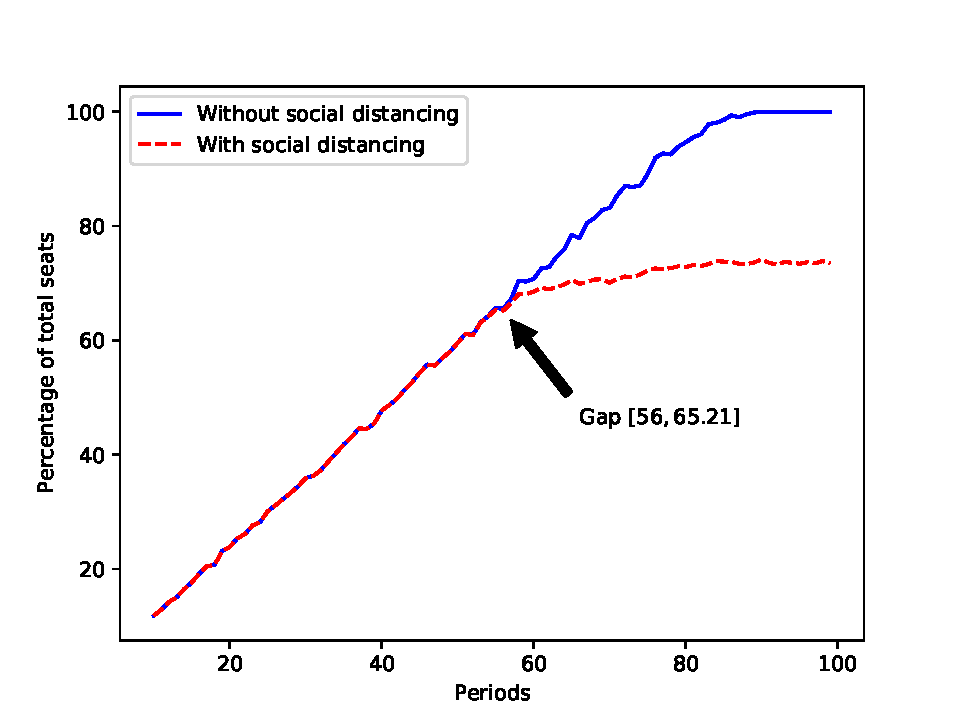
\includegraphics[width=0.48\textwidth]{./images/p1.pdf}}
            \subfigure[When $\gamma =1.9$]{
              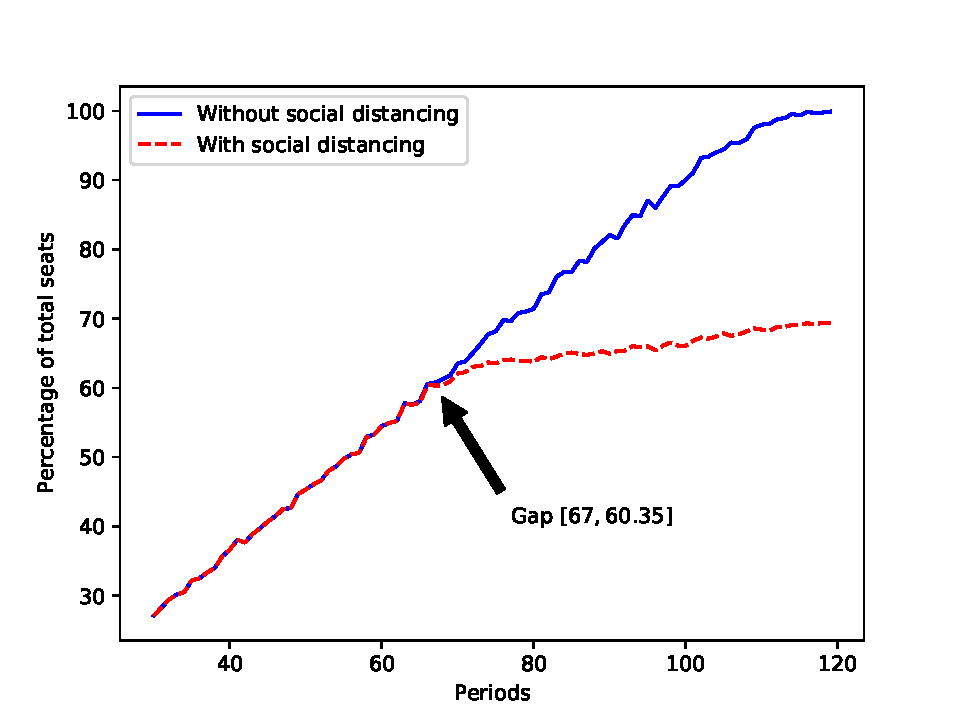
\includegraphics[width=0.48\textwidth]{./images/p2.pdf}}
          \end{figure}
        \scriptsize
        The gap point represents the first period where the number of people without social distancing is larger than that with social distancing and the gap percentage is the corresponding percentage of total seats.
    \end{frame}
      
    \begin{frame}{Estimation of Gap Point}
      \begin{figure}[ht]
        \centering
        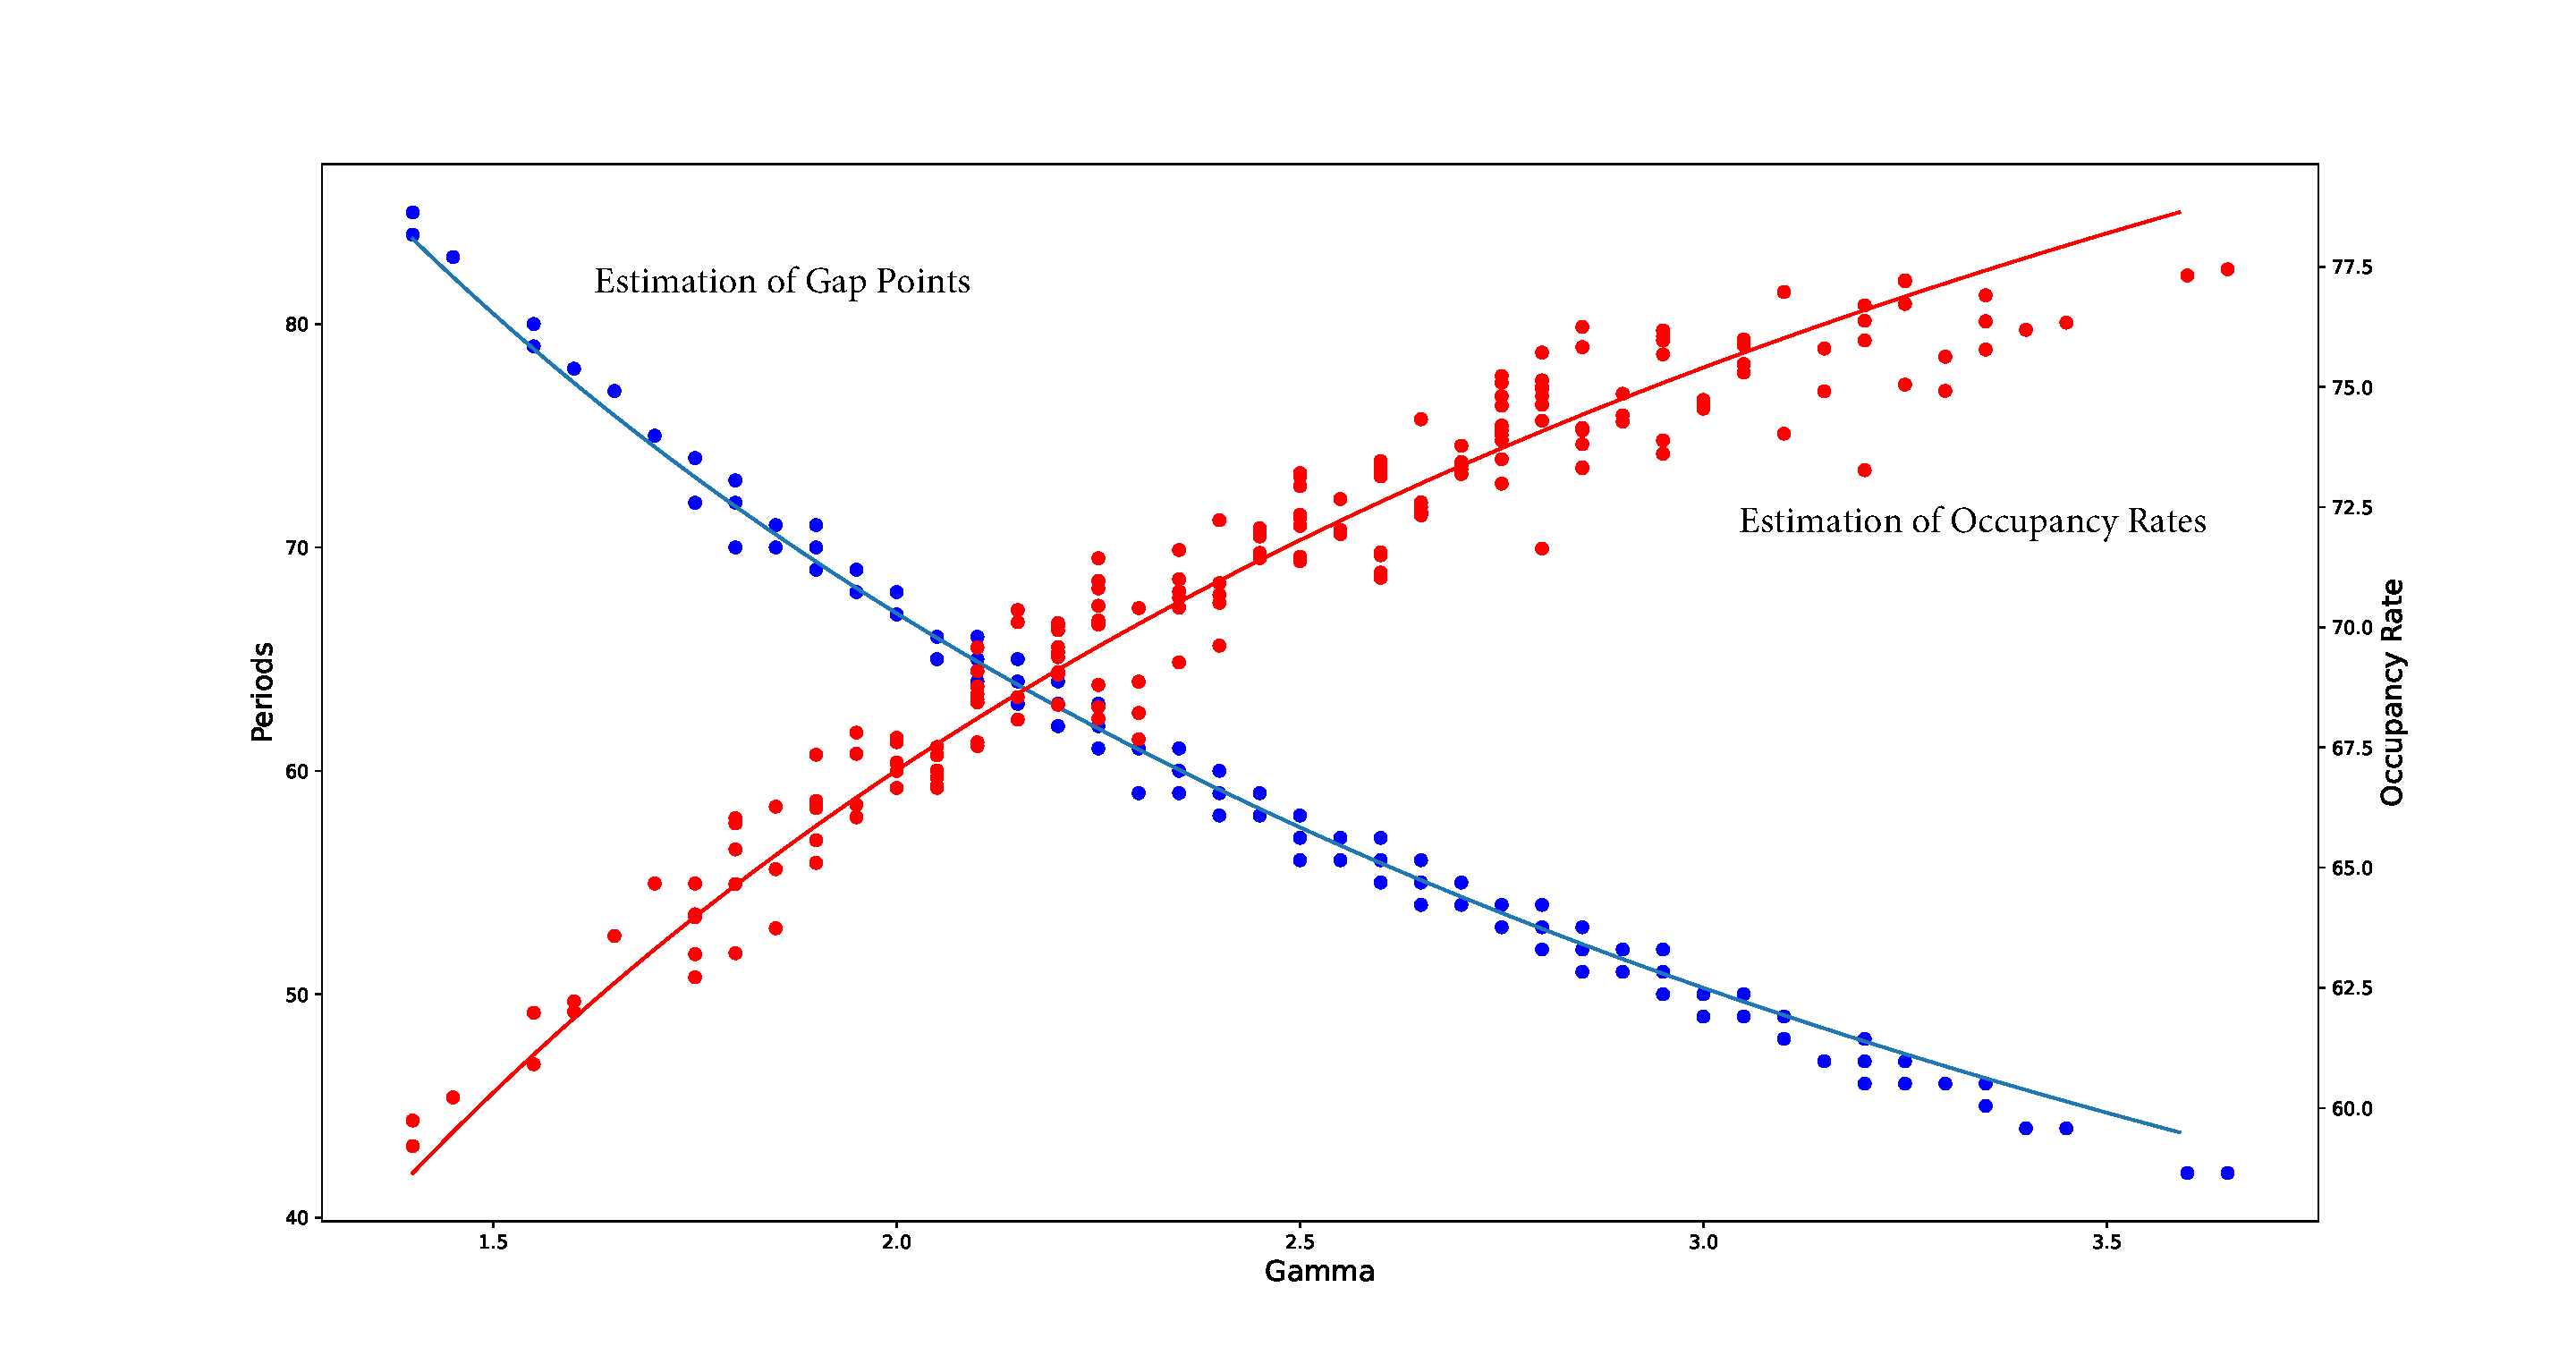
\includegraphics[width = 0.8\textwidth]{./images/gamma_estimation.pdf}
        \caption{Gap points with 200 probabilities}
    \end{figure}
    \scriptsize
    {\color{blue} Blue points}: period of the gap point.
    {\color{red} Red points}: occupancy rate of the gap point. 
    Gap points can be estimated.
    \end{frame}

    % We simulate 200 probabilities. For each probability, we run 100 instances to calculate the gap point and the corresponding occupancy rate. 
    
    % The point in the figure is the average of 100 instances. 
    % 


    \begin{frame}{Make A Later Allocation}
      This setting is particularly applicable to larger venues, such as stadiums, where an immediate decision is made when a group arrives, but the actual allocation of seats for that group is deferred to a later time.

      \vspace{0.5cm}

      The critical part is to make the decision, thus, we choose the following policies associated with relaxation forms.

      \vspace{0.5cm}

      Policies: 

      \begin{itemize}
        \item Dynamic programming based heuristic
        \item Bid-price control
      \end{itemize}
    \end{frame}

      \begin{frame}{Performances of Different Policies}
        \scriptsize
        \begin{table}[ht]
          \centering
          \begin{tabular}{|l|l|l|l|l|l|}
          \hline
           T & Probabilities &  DP1-L (\%) & Bid-L (\%) & DP1 (\%) & Bid (\%) \\
          \hline
          60  & [0.25, 0.25, 0.25, 0.25]  & 99.52 & 99.44 & 98.42 & 98.38 \\
          70  &   & 99.32 & 98.97 & 96.87 & 96.24 \\
          80  &   & 99.34 & 99.30 & 95.69 & 96.02 \\
          90  &   & 99.55 & 99.49 & 96.05 & 96.41  \\
          100 &   & 99.78 & 99.66 & 95.09 & 96.88 \\
          \hline
          60  & [0.25, 0.35, 0.05, 0.35]  & 99.50 & 99.37 & 98.26 & 98.25  \\
          70  &   & 99.40 & 98.97 & 96.62 & 96.06 \\
          80  &   & 99.46 & 99.24 & 96.01 & 95.89 \\
          90  &   & 99.59 & 99.35 & 96.77 & 96.62 \\
          100 &   & 99.77 & 99.61 & 97.04 & 97.14  \\
          \hline
          60  & [0.15, 0.25, 0.55, 0.05]  & 99.57 & 99.54 & 98.72 & 98.74 \\
          70  &   & 99.46 & 99.39  & 96.38 & 96.90 \\
          80  &   & 99.50 & 99.30  & 97.75 & 97.87 \\
          90  &   & 99.34 & 99.44  & 98.45 & 98.69 \\
          100 &   & 99.34 & 99.55  & 98.62 & 98.94 \\
          \hline
          \end{tabular}
        \end{table}

    \end{frame}

% !TEX root = sum1.tex
\section{Conclusion}
In conclusion, this paper addresses the problem of dynamic seat assignment with social distancing in the context of a pandemic. We propose a practical algorithm that balances seat utilization rates and the associated risk of infection to obtain a final seat planning that satisfies social distancing constraints when groups arrive. Our approach provides a comprehensive solution for optimizing seat assignments while ensuring the safety of customers. Our contributions include establishing a deterministic model to analyze the effects of social distancing when demand is known, using Benders decomposition methods to obtain the optimal solution for scenario-based stochastic programming, and developing a seat assignment policy for the dynamic situation. Our results demonstrate significant improvements over baseline strategies and provide guidance for developing attendance policies. Overall, our study highlights the importance of considering the operational significance behind social distancing and provides a new perspective for the government to adopt mechanisms for setting seat assignments to protect people in the post-pandemic era. Our study demonstrates the efficiency of obtaining the final seat planning using our proposed algorithm. The results indicate that our policy yields a seat planning that is very close to the optimal result. 

% Moreover, our analysis provides managerial guidance on how to set the occupancy rate and largest size of one group under the background of pandemic.


% \begin{table}[H]
%     \centering
%     \caption{xxxx}
%     \begin{tabular}{cccc}
%  \hline
%  a & aaaaaaaaa & aaaaaaaaaaaaaa & aaaaaaaaaaaaaaaaaaaa \\
%  \hline
%  a & \makebox[5ex][r]{123} & \makebox[6ex][r]{123456} & \makebox[6ex][r]{1}\\
%  a & \makebox[5ex][r]{12345} & \makebox[6ex][r]{123} & \makebox[6ex][r]{123} \\
%  a & \makebox[5ex][r]{1} & \makebox[6ex][r]{1234} & \makebox[6ex][r]{123456} \\
%  \hline
%  \end{tabular}
%  \end{table}

\bibliographystyle{elsarticle-harv}
\bibliography{refe}

% !TEX root = sum1.tex
\clearpage
% \section*{Proof}

\begin{pf}{Proof of Proposition \ref{sol_relax_deter}}
  First, we regard this problem as a special case of the Multiple Knapsack Problem (MKP), then we consider the LP relaxation of this problem.
  Treat the groups as the items, the rows as the knapsacks. There are $M$ types of items, the total number of which is $K = \sum_{i} d_i$, each item $k$ has a profit $p_k$ and weight $w_k$. 
  Sort these items according to profit-to-weight ratios $\frac{p_1}{w_1} \geq \frac{p_2}{w_2} \geq \ldots \geq \frac{p_K}{w_K}$. Let the break item $b$ be given by $b=\min \{j: \sum_{k=1}^j w_k \geq \tilde{L}\}$, where $\tilde{L} = \sum_{j=1}^{N} L_j$ is the total size of all knapsacks. 
  For the LP relaxation of \eqref{deter_upper}, the Dantzig upper bound \cite{dantzig1957discrete} is given by $u_{\mathrm{MKP}}=\sum_{j=1}^{b-1} p_j+\left(\tilde{L}-\sum_{j=1}^{b-1} w_j\right) \frac{p_b}{w_b}$. The corresponding optimal solution is to accept the whole items from $1$ to $b-1$ and fractional $(\tilde{L}-\sum_{j=1}^{b-1} w_j)$ item $b$. Suppose the item $b$ belong to type $\tilde{i}$, then for $i < \tilde{i}$, $x_{ij}^{*} = 0$; for $i > \tilde{i}$, $x_{ij}^{*} = d_{i}$; for $i = \tilde{i}$, $\sum_{j} x_{ij}^{*} = (\tilde{L} - \sum_{i = \tilde{i}+1}^{M} {d_i n_i})/ n_{\tilde{i}}$.
\end{pf}


\begin{pf}{Proof of Proposition \ref{lem_pattern}}
First, we construct a feasible pattern with the size of $qM + \max\{r-\delta, 0\}$, then we prove this pattern is largest. Let $L = n_M \cdot q + r$, where $q$ represents the number of times $n_M$ is selected (the quotient), and $r$ represents the remainder, indicating the number of remaining seats. It holds that $0 \leq r < n_M$. The number of people accommodated in the pattern $\bm{h}_{g}$ is given by $|\bm{h}_{g}| = q M + \max\{r-\delta, 0\}$. To establish the optimality of $|\bm{h}_{g}|$ as the largest number of people accommodated given the constraints of $L$, $\delta$, and $M$, we can employ a proof by contradiction.

Assuming the existence of a pattern $\bm{h}$ such that $|\bm{h}| > |\bm{h}_{g}|$, we can derive the following inequalities:

\begin{align*}
  & \sum_{i} (n_i - \delta) h_i > q M + \max\{r-\delta, 0\} \\
  \Rightarrow ~& L \geq \sum_{i} n_i h_i > \sum_{i} \delta h_i + q M + \max\{r-\delta, 0\} \\
  \Rightarrow ~& q(M + \delta) + r > \sum_{i} \delta h_i + q M + \max\{r-\delta, 0\} \\
  \Rightarrow ~& q \delta + r > \sum_{i} \delta h_i + \max\{r-\delta, 0\}
\end{align*}

\begin{enumerate}[(i)]
  \item When $r > \delta$, the inequality becomes $q+1 > \sum_{i} h_i$. It should be noted that $h_i$ represents the number of group type $i$ in the pattern. Since $\sum_{i} h_i \leq q$, the maximum number of people that can be accommodated is $q M < q M + r-\delta$.  
  \item When $r \leq \delta$, we have the inequality $q \delta + \delta \geq q \delta + r > \sum_{i} \delta h_i$. Similarly, we obtain $q+1 > \sum_{i} h_i$. Thus, the maximum number of people that can be accommodated is $q M$, which is not greater than $|\bm{h}_{g}|$.  
\end{enumerate}

Therefore, $\bm{h}$ cannot exist. The maximum number of people that can be accommodated in the largest pattern is $q M + \max\{r-\delta, 0\}$.
\end{pf}

\begin{pf}{Proof of Proposition \ref{prop_construction}}
  First of all, we demonstrate the feasibility of problem \eqref{improve_seat}. Given the feasible seat planning $\bm{H}$ and $\tilde{d}_{i} = \sum_{j=1}^{N} H_{ji}$, let $\hat{x}_{ij} = H_{ji}, i \in \mathcal{M}, j \in \mathcal{N}$, then $\{\hat{x}_{ij}\}$ satisfies the first set of constraints. Because $\bm{H}$ is feasible, $\{\hat{x}_{ij}\}$ satisfies the second set of constraints and integer constraints. Thus, problem \eqref{improve_seat} always has a feasible solution. 
  
  Suppose there exists at least one pattern $\bm{h}$ is neither full nor largest in the optimal seat planning obtained from problem \eqref{improve_seat}. Let $\beta = L - \sum_{i} n_{i} h_{i}$, and denote the smallest group type in pattern $\bm{h}$ by $k$. If $\beta \geq n_1$, we can assign at least $n_1$ seats to a new group to increase the objective value. Thus, we consider the situation when $\beta < n_1$. If $k =M$, then this pattern is largest. When $k< M$, let $h^{1}_{k} = h_{k} -1$ and $h^{1}_{j} = h_{j} +1$, where $j = \min\{M, \beta + k\}$. In this way, the constraints will still be satisfied but the objective value will increase when the pattern $\bm{h}$ changes. Therefore, by contradiction, problem \eqref{improve_seat} always generate a seat planning composed of full or largest patterns.
\end{pf}


\begin{pf}{Proof of Proposition \ref{prop_solution}}
  In any optimal solution where one of the corresponding patterns is neither full or largest, we can utilize the conclusion of Proposition \ref{prop_construction} to obtain a seat planning that is composed of full or largest patterns meanwhile the constraints of SSP are still satisfied.
\end{pf}


\begin{pf}{Proof of Lemma \ref{feasible_region}}
Note that $\mathbf{f}^{\intercal} = [-\mathbf{1},~\mathbf{0}]$ and $\mathbf{V} = [\mathbf{W},~\mathbf{I}]$. Based on this, we can derive the following inequalities: $\bm{\alpha}^{\intercal} \mathbf{W} \geq -\mathbf{1}$ and $\bm{\alpha}^{\intercal} \mathbf{I} \geq \mathbf{0}$. According to the expression of $\mathbf{W}$ and $\mathbf{I}$, we can deduce that $0 \leq \alpha_i \leq \alpha_{i-1} +1$ for $i \in \mathcal{M}$ by letting $\alpha_0 = 0$. These inequalities indicate that the feasible region is nonempty and bounded. For $i \in \mathcal{M}$, $\alpha_{i}$ is only bounded by $\alpha_{i-1}+1$ and $0$, thus, all extreme points within the feasible region are integral.
\end{pf}

\begin{pf}{Proof of Proposition \ref{optimal_sol_sub_dual}}
  According to the complementary slackness property, we can obtain the following equations
  \begin{align*}
    & \alpha_{i} (d_{i0} - d_{i \omega} - y_{i \omega}^{+} + y_{i+1, \omega}^{+} + y_{i \omega}^{-}) = 0, i =1,\ldots, M-1 \\
    & \alpha_{i} (d_{i0} - d_{i \omega} - y_{i \omega}^{+}+ y_{i \omega}^{-}) = 0, i = M \\
    & y_{i \omega}^{+}(\alpha_{i} - \alpha_{i-1}-1) = 0, i =1,\ldots, M \\
    & y_{i \omega}^{-} \alpha_{i} = 0, i =1,\ldots, M.
  \end{align*}
  

    When $y_{i \omega}^{-} >0$, we have $\alpha_{i} =0$. When $y_{i \omega}^{+} >0$, we have $\alpha_{i} = \alpha_{i-1} +1$. When $y_{i \omega}^{+} = y_{i \omega}^{-} = 0$, let $\Delta d = d_{\omega} - d_0$,
    \begin{itemize}
      \item if $i = M$, $\Delta d_{M} =0$, the value of objective function associated with $\alpha_{M}$ is always $0$, thus we have $0 \leq \alpha_{M} \leq \alpha_{M-1}+1$;
      \item if $i < M$, we have $y_{i+1, \omega}^{+} = \Delta d_{i} \geq 0$.
      \begin{itemize}
        \item If $y_{i+1, \omega}^{+} > 0$, the objective function associated with $\alpha_i$ is $\alpha_{i} \Delta d_{i} = \alpha_{i} y_{i+1, \omega}^{+}$, thus to minimize the objective value, we have $\alpha_i =0$.
        \item If $y_{i+1, \omega}^{+} = 0$, we have $0 \leq \alpha_{i} \leq \alpha_{i-1} +1$.
      \end{itemize}
    \end{itemize}
  \end{pf}

  \begin{pf}{Proof of Proposition \ref{one_ep_feasible}}
    Suppose we have one extreme point $\bm{\alpha}_{\omega}^{0}$ for each scenario. Then we have the following problem.
    \begin{equation}\label{lemma_eq}
      \begin{aligned}
        \max \quad & \mathbf{c}^{\intercal} \mathbf{x} + \sum_{\omega \in \Omega} p_{\omega} z_{\omega} \\
        \text {s.t.} \quad & \mathbf{n} \mathbf{x} \leq \mathbf{L} \\
        & (\bm{\alpha}_{\omega}^{0})^{\intercal}\mathbf{d}_{\omega} \geq (\bm{\alpha}_{\omega}^{0})^{\intercal} \mathbf{x} \mathbf{1} + z_{\omega}, \forall \omega \\
         & \mathbf{x} \in \mathbb{N}^{M \times N}
      \end{aligned}
    \end{equation}
    Problem \eqref{lemma_eq} reaches its maximum when $(\bm{\alpha}_{\omega}^{0})^{\intercal}\mathbf{d}_{\omega} = (\bm{\alpha}_{\omega}^{0})^{\intercal} \mathbf{x} \mathbf{1} + z_{\omega}, \forall \omega$. Substitute $z_{\omega}$ with these equations, we have 
    \begin{equation}\label{lemma_eq2}
      \begin{aligned}
        \max \quad & \mathbf{c}^{\intercal} \mathbf{x} - \sum_{\omega}p_{\omega}(\bm{\alpha}_{\omega}^{0})^{\intercal} \mathbf{x} \mathbf{1} + \sum_{\omega} p_{\omega} (\bm{\alpha}_{\omega}^{0})^{\intercal} \mathbf{d}_{\omega} \\
        \text {s.t.} \quad & \mathbf{n} \mathbf{x} \leq \mathbf{L} \\
        & \mathbf{x} \in \mathbb{N}^{M \times N}
      \end{aligned}
    \end{equation}
    Notice that $\mathbf{x}$ is bounded by $\mathbf{L}$, then the problem \eqref{lemma_eq} is bounded. Adding more constraints will not make the optimal value larger. Thus, RBMP is bounded. 
  \end{pf}
  


\begin{pf}{Proof of Lemma \ref{bid-price}}
According to the Proposition \ref{sol_relax_deter}, the aggregate optimal solution to LP relaxation of problem \eqref{deter_upper} takes the form $x e_{\tilde{i}} + \sum_{i=\tilde{i}+1} ^{M} d_{i} e_{i}$, then according to the complementary slackness property, we know that $z_1, \ldots, z_{\tilde{i}} = 0$. This implies that $\beta_j \geq \frac{n_i - \delta}{n_i}$ for $i = 1,\ldots, \tilde{i}$. Since $\frac{n_i - \delta}{n_i}$ increases with $i$, we have $\beta_j \geq \frac{n_{\tilde{i}} - \delta}{n_{\tilde{i}}}$. Consequently, we obtain $z_{i} \geq n_i - \delta - n_i \frac{n_{\tilde{i}} - \delta}{n_{\tilde{i}}} = \frac{\delta(n_i-n_{\tilde{i}})}{n_{\tilde{i}}}$ for $i = h+1, \ldots, M$.
  
Given that $\mathbf{d}$ and $\mathbf{L}$ are both no less than zero, the minimum value will be attained when $\beta_j = \frac{n_{\tilde{i}} - \delta}{n_{\tilde{i}}}$ for all $j$, and $z_i = \frac{\delta(n_i-n_{\tilde{i}})}{n_{\tilde{i}}}$ for $i = \tilde{i}+1, \ldots, M$.  
\end{pf}

\newpage


\end{document}
